%----------------------------------------------
% PACCHETTI
%----------------------------------------------
\documentclass[12pt,a4paper]{article}
\usepackage[a4paper]
\usepackage[T1]{fontenc}
\usepackage[utf8]{inputenc}
\usepackage[italian]{babel}
\usepackage{lipsum}
\usepackage{hyperref}
\usepackage{lastpage}
\usepackage{fancyhdr}
\usepackage{graphicx}
\usepackage{url}
\usepackage{geometry}
\usepackage{xcolor}
\usepackage{amssymb}
\usepackage{amsmath}
\usepackage{booktabs}

%----------------------------------------------
% NUOVI COMANDI
%----------------------------------------------
\newcommand{\Sep}{\vspace{1.5em}}
\newcommand{\MidSep}{\vspace{1em}}
\newcommand{\SmallSep}{\vspace{0.5em}}

\newcommand{\numberset}{\mathbb}
\newcommand{\N}{\numberset{N}} 
\newcommand{\Z}{\numberset{Z}}
\newcommand{\Q}{\numberset{Q}}
\newcommand{\R}{\numberset{R}}
\newcommand{\C}{\numberset{C}}
%----------------------------------------------
% INTESTAZIONE  E PIE DI PAGINA
%----------------------------------------------
\pagestyle{myheadings}
\pagestyle{fancy}
\fancyhf{}
\hypersetup{hidelinks}

\headsep= 20mm

\renewcommand{\headrulewidth}{2pt}
\renewcommand{\footrulewidth}{2pt}

\lhead{
\includegraphics[width=0.4\columnwidth]{img/units_logo}}
\rhead{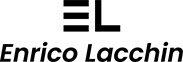
\includegraphics[width=0.3\columnwidth]{img/logo_black}}\lfoot{© Enrico Lacchin | \url{www.enricolacchin.com}}
\cfoot{}
\rfoot{\thepage}

\leftskip 0.0pt

%----------------------------------------------
% INIZIO DOCUMENTO
%----------------------------------------------
\begin{document}

%----------------------------------------------
% TITOLO
%----------------------------------------------
\pagenumbering{gobble}

\small{Enrico Lacchin}

\MidSep
\textbf{\LARGE{Logistica}}

\MidSep
\textit{\Large{Appunti}}
\Sep

\begin{center}
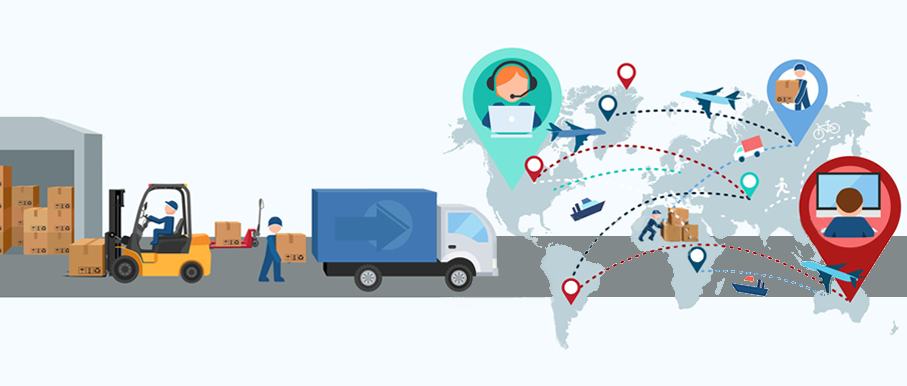
\includegraphics[width=1\columnwidth]{img/logistica.png}
\end{center}

\vfill
Materia: Logistica

Docente: Luca Coslovich

%----------------------------------------------
% INDICE
%----------------------------------------------

\clearpage
\pagenumbering{roman}
\setcounter{page}{1}
\tableofcontents

%----------------------------------------------
% INIZIO CAPITOLI
%----------------------------------------------
%CAPITOLO 1
\clearpage

\pagenumbering{arabic}
\setcounter{page}{1}

\section{Problema del Trasporto}
\begin{center}
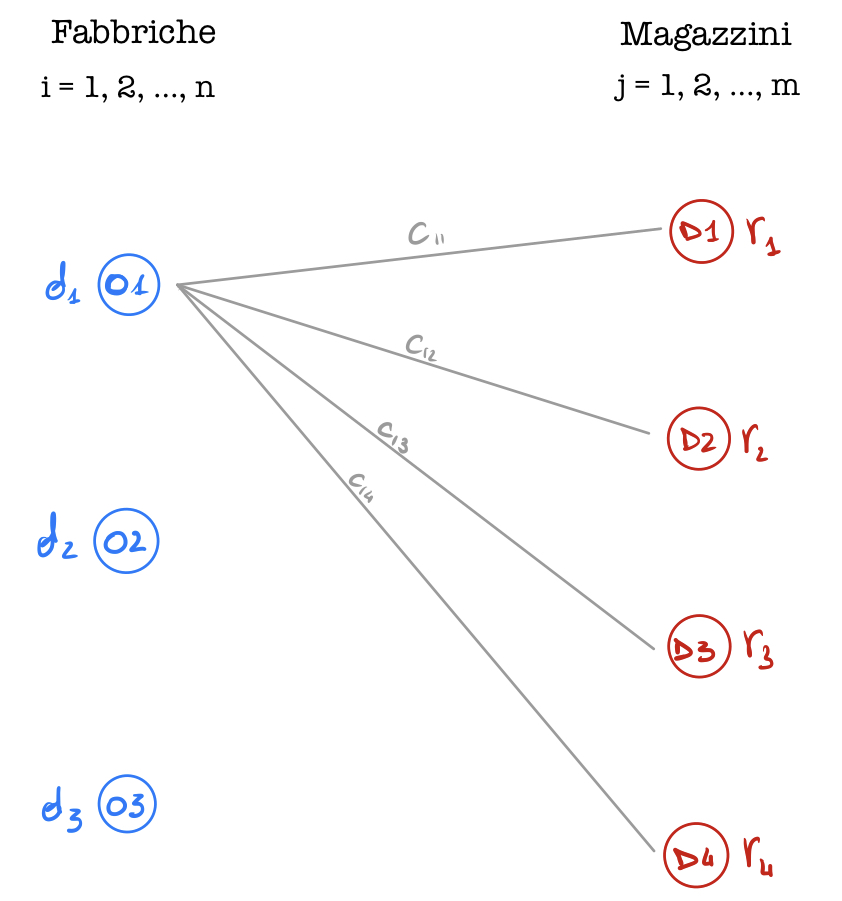
\includegraphics[width=0.6\columnwidth]{img/trasporto.jpeg}
\end{center}
\subsection{Formulazione Matematica}
\paragraph{Variabili decisionali} $$x_{ij} = \text{quantità trasportata da $O_i$ a $D_j$}$$
\paragraph{Funzione Obiettivo} $$min\ z = \sum_i^n \sum_j^m x_{ij}\cdot c_{ij}$$
\paragraph{Vincoli} \begin{itemize}
\item $\sum_j x_{ij} \leq d_i, \ \ \forall i = 1, \dots, n$
\item $\sum_i x_{ij} \geq r_j, \ \ \forall j = 1, \dots, n$
\item $x_{ij} \geq 0, \ \ \forall i, j$
\end{itemize}

\textbf{Nota Bene}: \begin{itemize}
\item Se $\sum_i d_i \leq \sum_j r_j$ il problema \textcolor{red}{NON è ammissibile}
\item Se $\sum_i d_i \geq \sum_j r_j$ il problema \textcolor{ao}{è ammissibile}
\item Se $\sum_i d_i > \sum_j r_j$ il problema \textcolor{ao}{è ammissibile}, ma aggiungo un magazzino $D_{m+1}$ nel quale la sua richiesta $r_{m+1} = \sum_i d_i - \sum_j r_j$ e il suo costo $c_{ij} = 0$
\end{itemize}

\noindent
Un problema del trasporto è costituito da $N \times M$ variabili, $N+M$ vincoli funzionali (di cui $N+M - 1$ indipendenti tra loro) e $N \times M - (N+M-1) = (N-1)(M-1)$ variabili fuori base.

\subsection{Proprietà: Totale Unimodularità}
Siano tutte le disponibilità intere e tutte le richiesta intere\\
\textbf{Tesi}: Esiste una soluzione ottima intera.
\begin{equation*}
\begin{array}{c}
d_i \ intero, \ \ \forall i\\
r_j \ intero, \ \ \forall j
\end{array} \Bigg\} \Rightarrow \exists \ \text{soluzione ottima intera}
\end{equation*}
$\Rightarrow$ La regione ammissibile è tale per cui tutti i vertici stanno su punti interi.\\
\\
\textbf{Osservazione}: Se il problema è equilibrato posso scrivere i vincoli con l'uguaglianza (=)

\subsection{Matrice dei trasporti (con esempio)}
Sia dato il seguente problema:
\begin{itemize}
\item Le disponibilità $i$ delle fabbriche sono le seguenti: $O_1=40, \ O_2=60,\ O_3=90, \ O_4=50$
\item Le richieste $j$ dei magazzini sono le seguenti: $D_1=30, \ D_2=40,\ D_3=70, \ D_4=40, \ D_5 = 60$
\end{itemize}
Prima del riempimento la matrice dei trasporti sarà:
\begin{center}
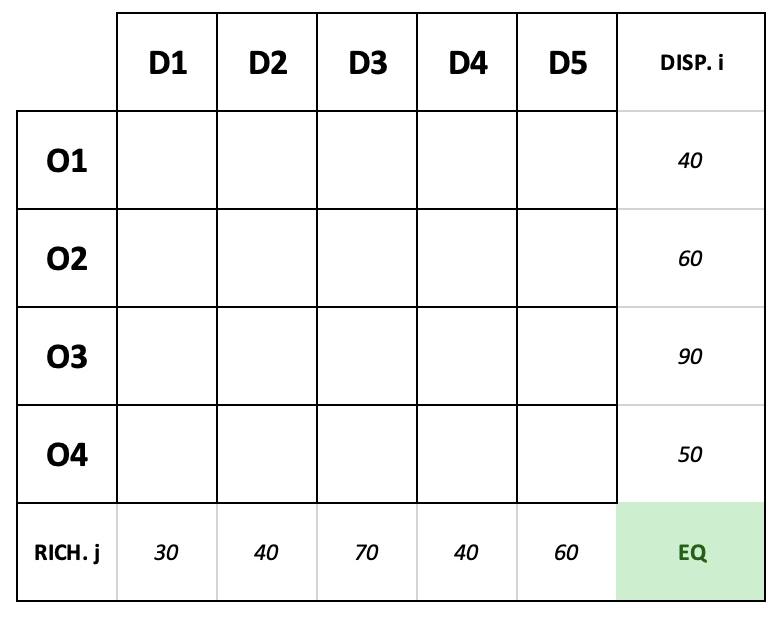
\includegraphics[width=0.4\columnwidth]{img/mat_trasporti_clean.png}
\end{center}
Vado a riempire la matrice dei trasporti seguendo il metodo "\textbf{Angolo di N-W}" e ottengo:
\begin{center}
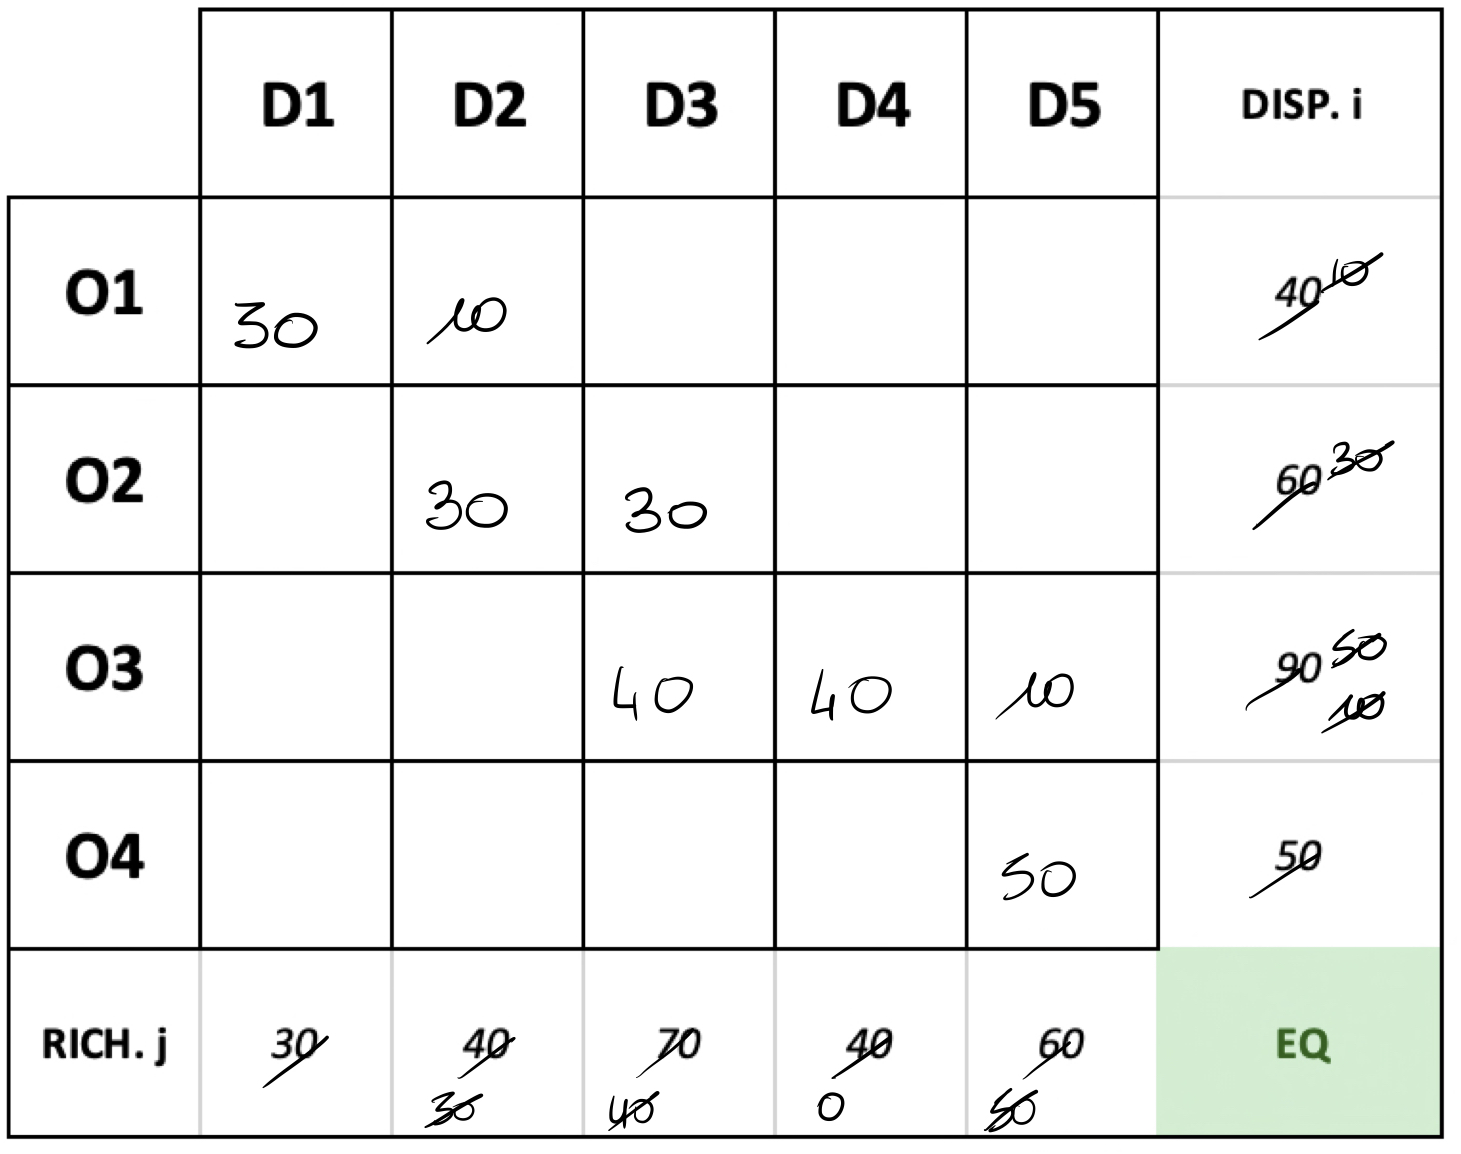
\includegraphics[width=0.4\columnwidth]{img/mat_trasporti_nw.jpeg}
\end{center}
Se volessi trasportare $30$ in  $O_4/D_1$ e farlo entrare in base cosa dovrei fare?
\begin{center}
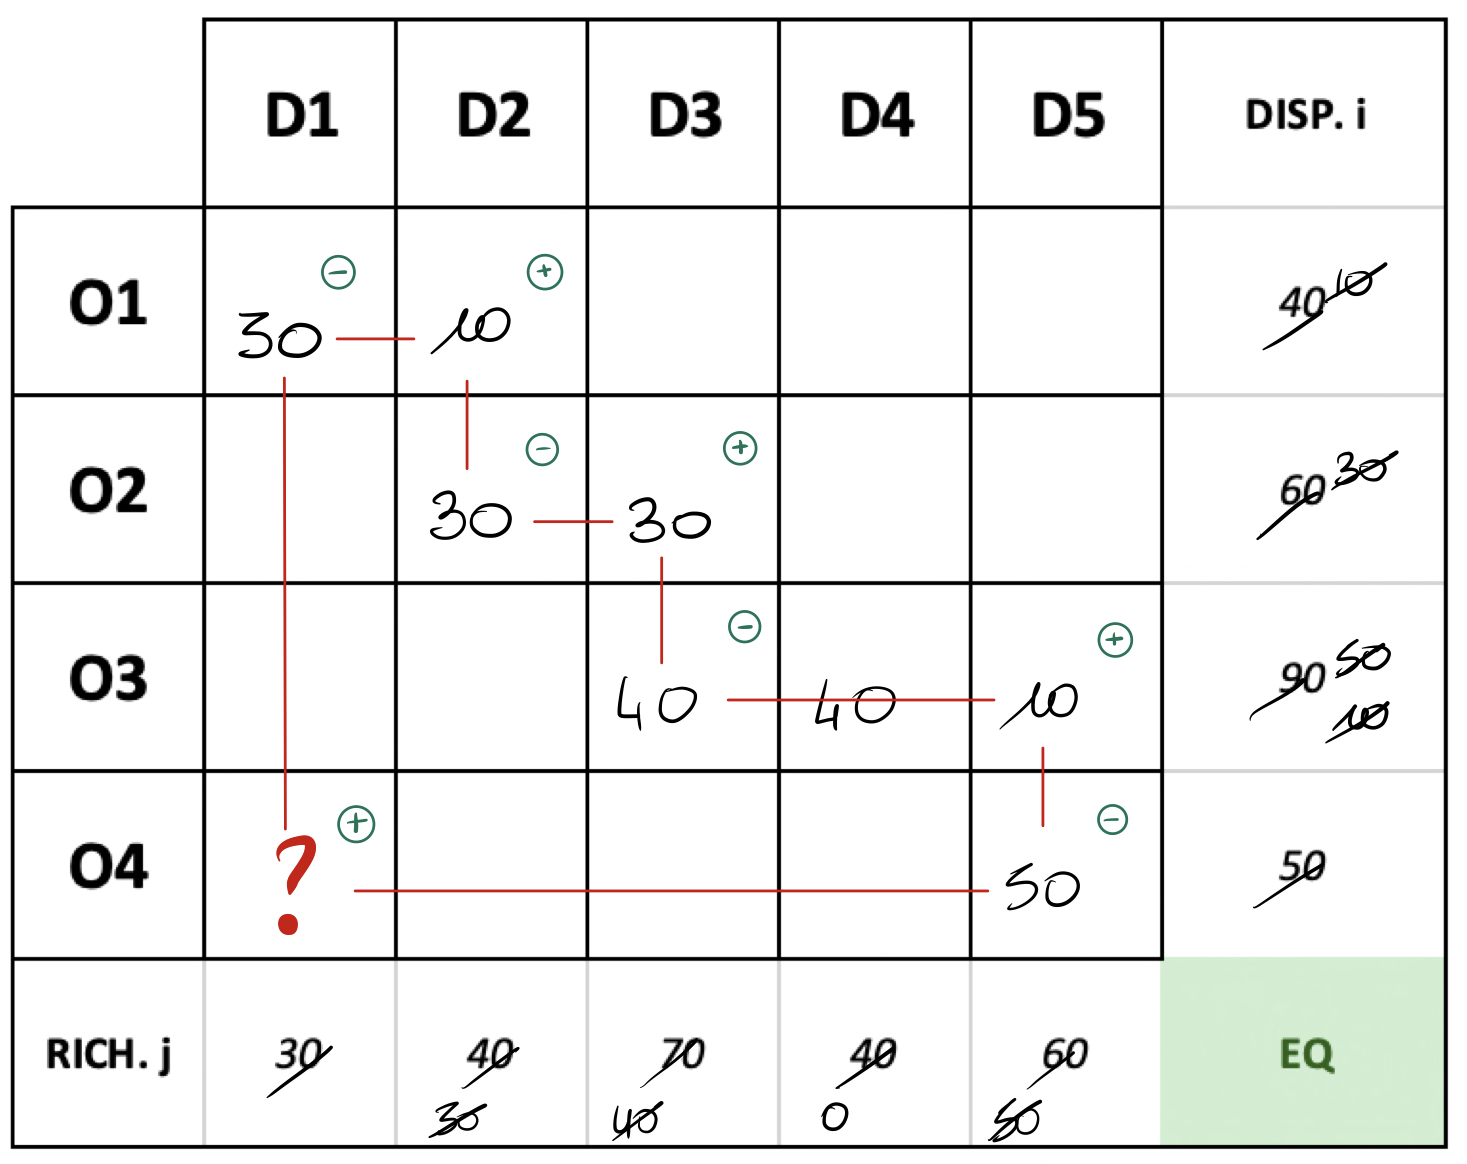
\includegraphics[width=0.4\columnwidth]{img/mat_trasporti_O4D1.jpeg}
\end{center}
\begin{enumerate}
\item \textbf{Perché ho trasportato 30?} Ho trasportato 30 perché il $min\{30,30,40,50\}$ che sono i valori che poi andrò a sottrarre.
\item \textbf{Perché questo percorso?} è l'unico percorso disponibile, per trovarlo devo:
\begin{itemize}
\item Mettere una "x" sulle variabili in base $\blacksquare$
\item Mettere una "x" sulla variabile fuori base che voglio far entrare in base $\textcolor{red}{\blacksquare}$
\item Cancellare le righe / colonne con una sola "x" 
\item Vedere qual è il percorso (muovendomi in verticale e orizzontale) che mi permette di chiudere il ciclo. $\textcolor{bluel}{\blacksquare}$
\end{itemize}
\begin{center}
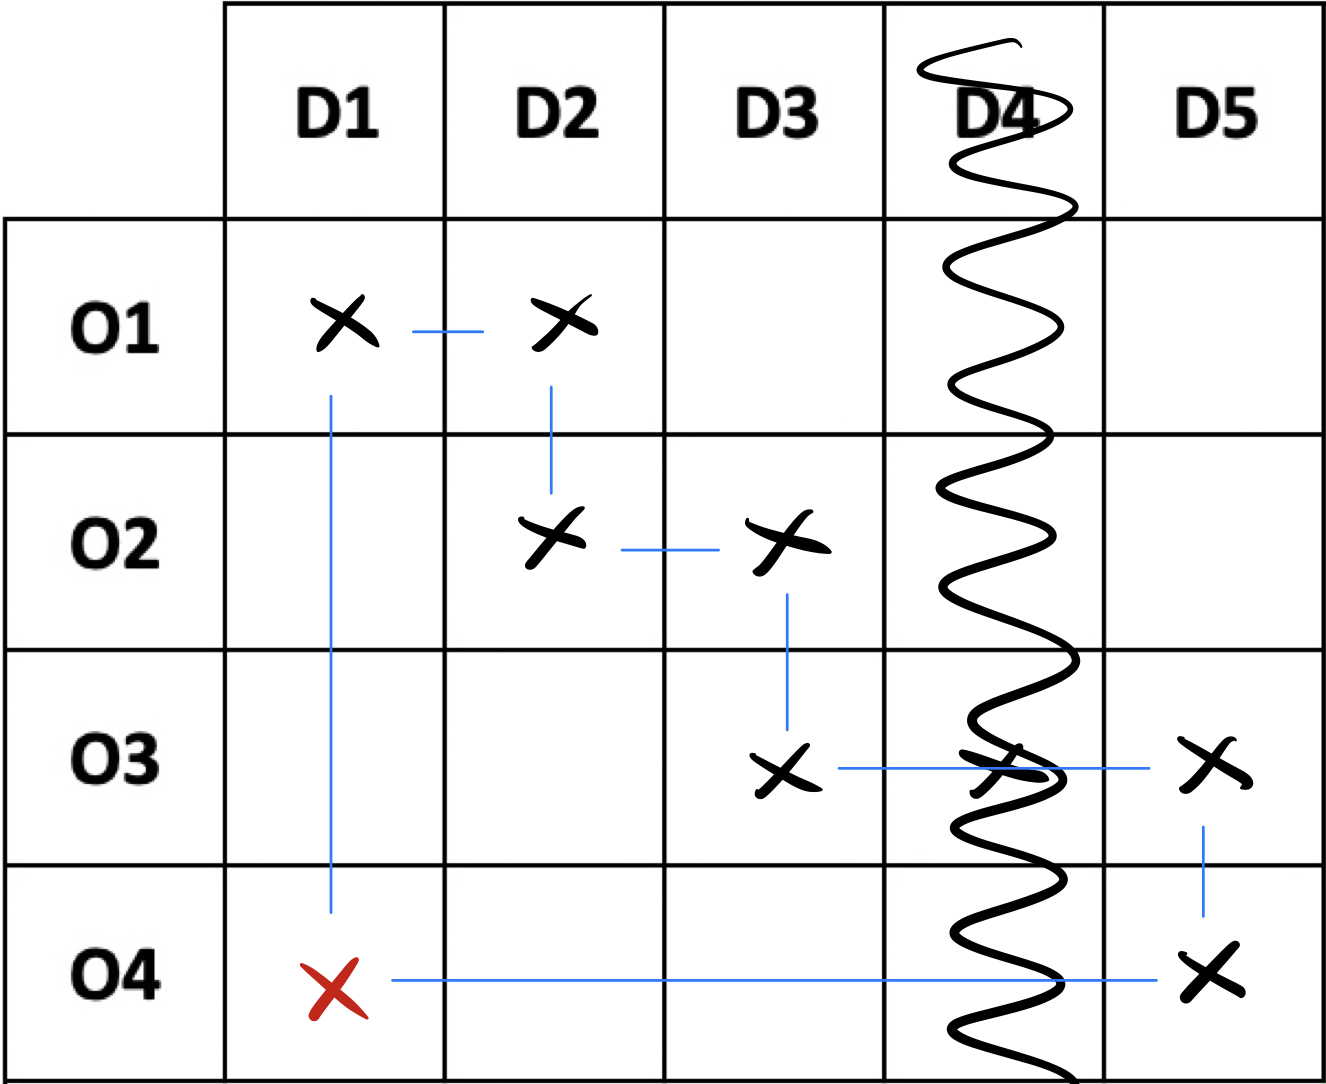
\includegraphics[width=0.4\columnwidth]{img/stepping_stone_1.jpeg}
\end{center}
\item \textbf{Conviene o non conviene?} Per dire se conviene o non conviene fare questo spostamento bisogna introdurre il concetto di "\textbf{Costo Marginale Unitario}[$C_M$]" che equivale alla somma/sottrazione dei costi unitari lungo il percorso scelto. Nel nostro caso
$$C_M = c_{41} - c_{11} + c_{12} - c_{22} + c_{23} - c_{33} + c_{35} - c_{45}$$
\begin{itemize}
\item Se $C_M < 0$  \textcolor{ao}{conviene}
\item Se $C_M > 0$  \textcolor{red}{NON conviene}
\item Se $C_M = 0$  è indifferente
\end{itemize}
\end{enumerate}

\subsection{Esempio pratico}
\begin{center}
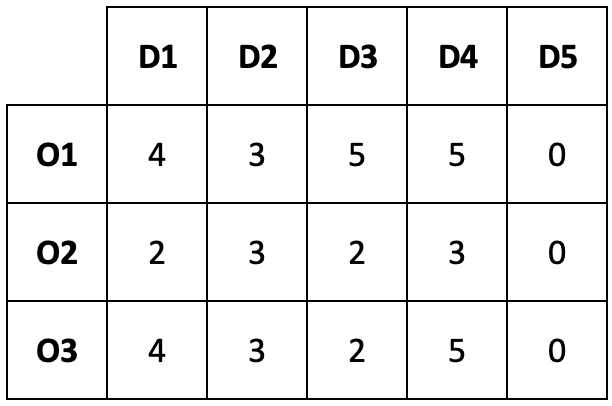
\includegraphics[width=0.4\columnwidth]{img/prob_trasporto_costi.png}\\
Tabella Costi\\
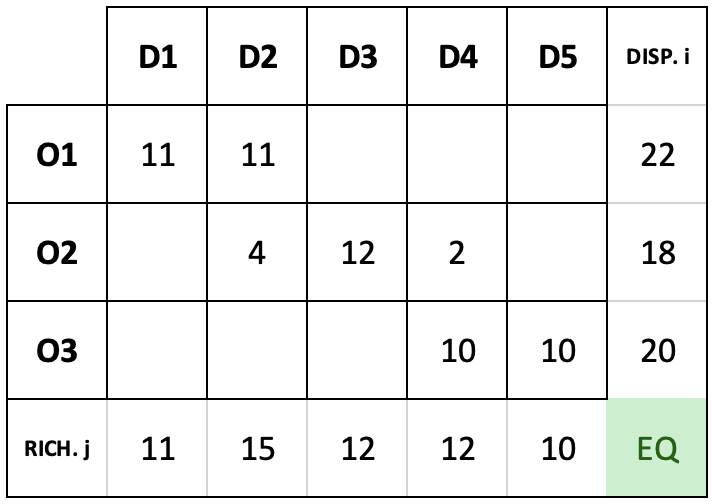
\includegraphics[width=0.4\columnwidth]{img/prob_trasporto_DR.png}\\
Tabella Domanda e Richiesta (riempita con metodo "Angolo di N-W")
\end{center}
$\textcolor{red}{Costo} = 11\cdot 4 + 11\cdot 3+ 4\cdot 3 +  12\cdot 2 + 2\cdot 3+ 10\cdot 5+10\cdot 0 = 169$\\
Possiamo spendere di meno?
\begin{itemize}
\item \textbf{O2/D1} $\rightarrow \ \  \begin{array}{l}\text{Quanto trasporto: 4} = min\{11, 4\}\\ C_M = 2- 4 + 3 - 4 = -2 \Rightarrow \textcolor{ao}{CONVIENE}\\Nuovo\ costo = costo - C_M \cdot quantita = 161\end{array} \ \ \ \textcolor{ao}{\blacksquare}$\\
\begin{center}
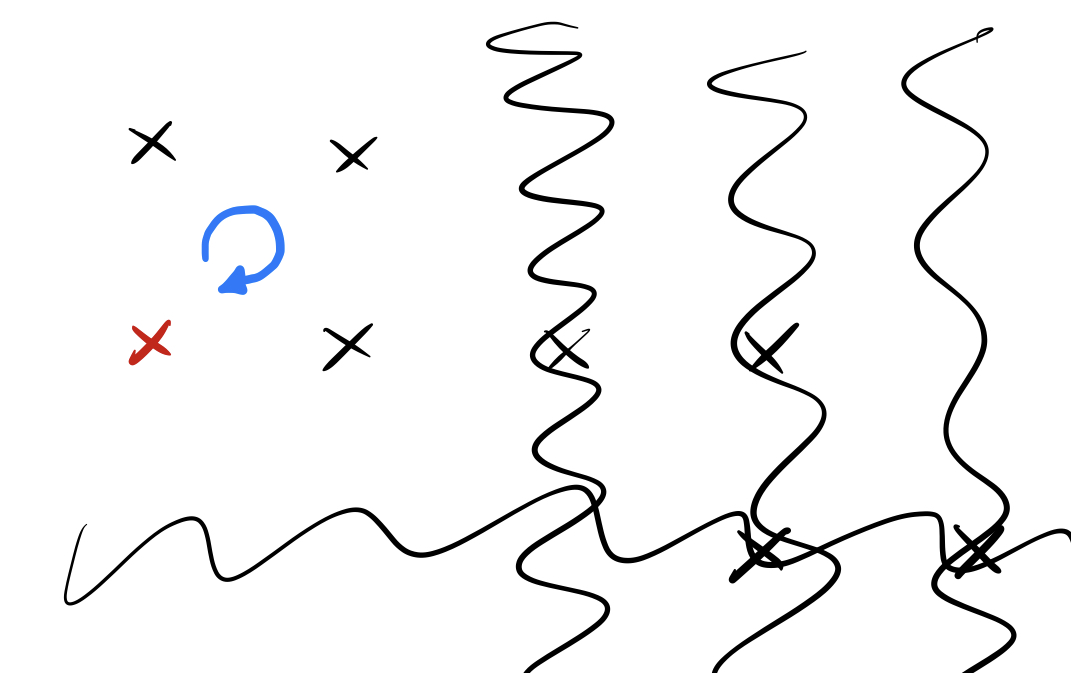
\includegraphics[width=0.3\columnwidth]{img/prob_trasporto_O2D1.jpeg}
\end{center}
\item \textbf{O3/D2} $\rightarrow \ \ C_M = 3- 3 + 4 - 2+3-5 = 0 \Rightarrow Indifferente$
\item \textbf{O1/D3} $\rightarrow \ \ C_M = 5-2+2-4 = 1 \Rightarrow \textcolor{red}{NON\ CONVIENE}$
\item \textbf{O1/D4} $\rightarrow \ \ C_M =  0 \Rightarrow Indifferente$
\item \textbf{O1/D5} $\rightarrow \ \ C_M =  0 \Rightarrow Indifferente$
\item \textbf{O2/D5} $\rightarrow \ \ C_M =  2 \Rightarrow \textcolor{red}{NON\ CONVIENE}$
\item \textbf{O2/D2} $\rightarrow \ \ C_M =  2 \Rightarrow \textcolor{red}{NON\ CONVIENE}$
\item \textbf{O3/D1} $\rightarrow \ \ C_M =  0 \Rightarrow Indifferente$
\item \textbf{O3/D3} $\rightarrow \ \  \begin{array}{l}\text{Quanto trasporto: 10}\\ C_M = -2 \Rightarrow \textcolor{ao}{CONVIENE}\\Nuovo\ costo = 161 - 10\cdot 2 = 141\end{array} \ \ \ \textcolor{bluel}{\blacksquare}$
\item \textbf{O1/D5} $\rightarrow \ \  \begin{array}{l}\text{Quanto trasporto: 2}\\ C_M = -2 \Rightarrow \textcolor{ao}{CONVIENE}\\Nuovo\ costo = 141 - 2\cdot 2 = 137\end{array} \ \ \ \textcolor{red}{\blacksquare}$
\end{itemize}
Arrivo alla soluzione ottima:
\begin{center}
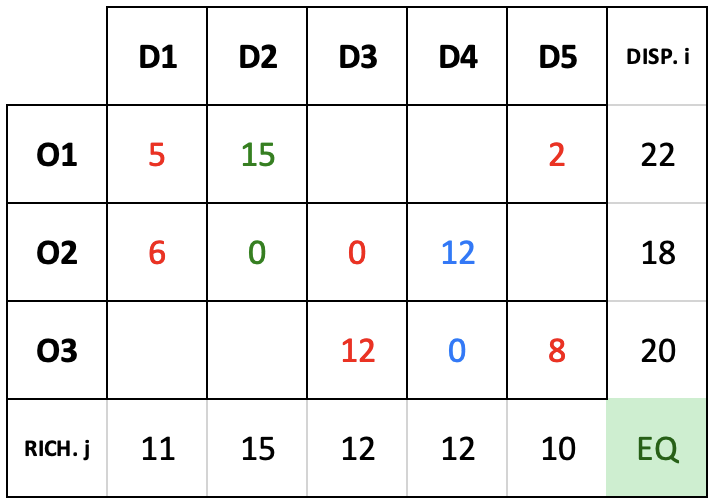
\includegraphics[width=0.4\columnwidth]{img/prob_trasporto_sol.png}
\end{center}

\subsection{Tecnica del "Big M"}
$$C_{N+1,j} = M >> \dots$$
dove:\begin{itemize}
\item $C_{N+1,j}$ = Costo unitario elevato
\item $\dots$ = Altri parametri in gioco
\end{itemize}
In questo caso il $\text{costo finale del trasporto} = costo' - D_{N+1}\cdot M \rightarrow$ cosi posso studiare un problema inizialmente non ammissibile.\\
{\scriptsize $D_{N+1}$ mi rappresenta quella che è una disponibilità fittizia.}

\subsection{Problema Degenere}
Supponiamo di trovare un problema in cui:
\begin{center}
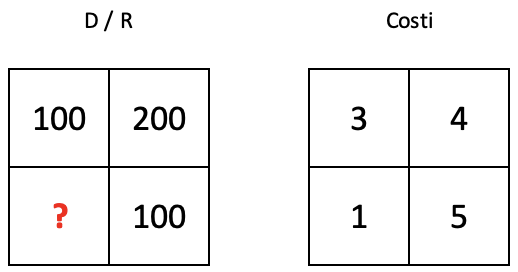
\includegraphics[width=0.4\columnwidth]{img/pb_trasporto_deg.png}
\end{center}
$\begin{array}{l}C_M = 1-3+4-5=-3 < 0\\
min\{100, 100\} = 100\end{array}$\\
\\
\begin{tabular}{l l}
\parbox{0.6\columnwidth}{Iterando l'algoritmo di Stepping Stone ottengo:} &
\parbox{\textwidth}{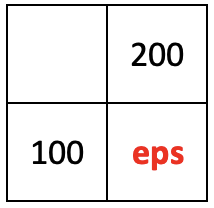
\includegraphics[width=0.2\columnwidth]{img/pb_trasporto_deg_ss.png}}\\
\end{tabular}
\\
\textcolor{red}{\textbf{eps}} è in base ma con valore nullo $\rightarrow$ è utilizzabile in successive iterazioni di stepping stone $\Rightarrow$ tale soluzione si dice degenere.

\subsection{Più soluzioni ottime}
Una soluzione è ottima quando tutti i costi marginali alternativi provati con altre interazioni di stepping stone sono $>0$ (non ce ne sono altri $<0$)\\
$\Rightarrow$ se ho due soluzioni ottime $\rightarrow$ ce ne sono infinite (non è detto che siano tutte intere)

\subsection{Metodo del minimo costo}
\begin{center}
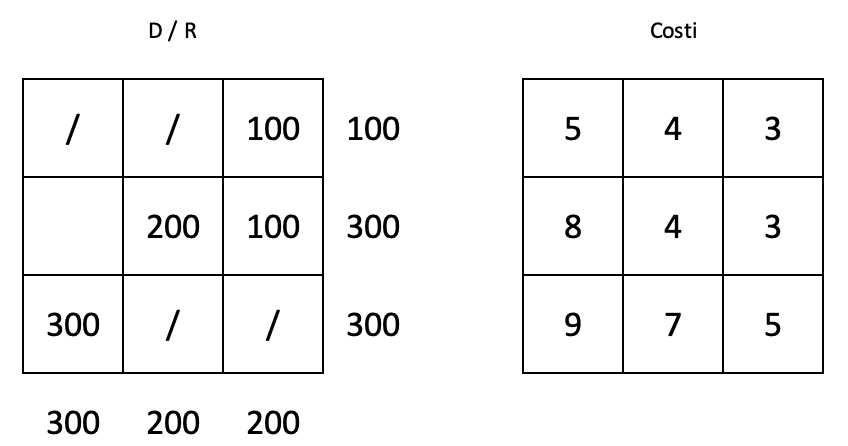
\includegraphics[width=0.5\columnwidth]{img/pb_trasporto_mincosto.png}
\end{center}
Noto che se applicassi il metodo "Angolo di N-W" il costo sarebbe pari a $4'200$, invece partendo dalle caselle con costo più basso il costo si abbassa a $4'100$

\subsection{Metodo di Vogel [VAM]}
\textbf{Costi di opportunità}: differenza tra i due costi più bassi.\\
\\
\textbf{Algoritmo}:
\begin{enumerate}
\item Per ogni riga/colonna determino il costo di opportunità
\item Scelgo la riga/colonna con il costo di opportunità maggiore
\item Per la riga/colonna scelta trasporto il più possibile
\item Elimino righe/colonne "sature"
\item Itero $\Rightarrow$ ricalcolo i costi di opportunità
\item Vai al punto 2
\end{enumerate}
Applicando il "Metodo di Vogel" ottengo la tabella seguente
\begin{center}
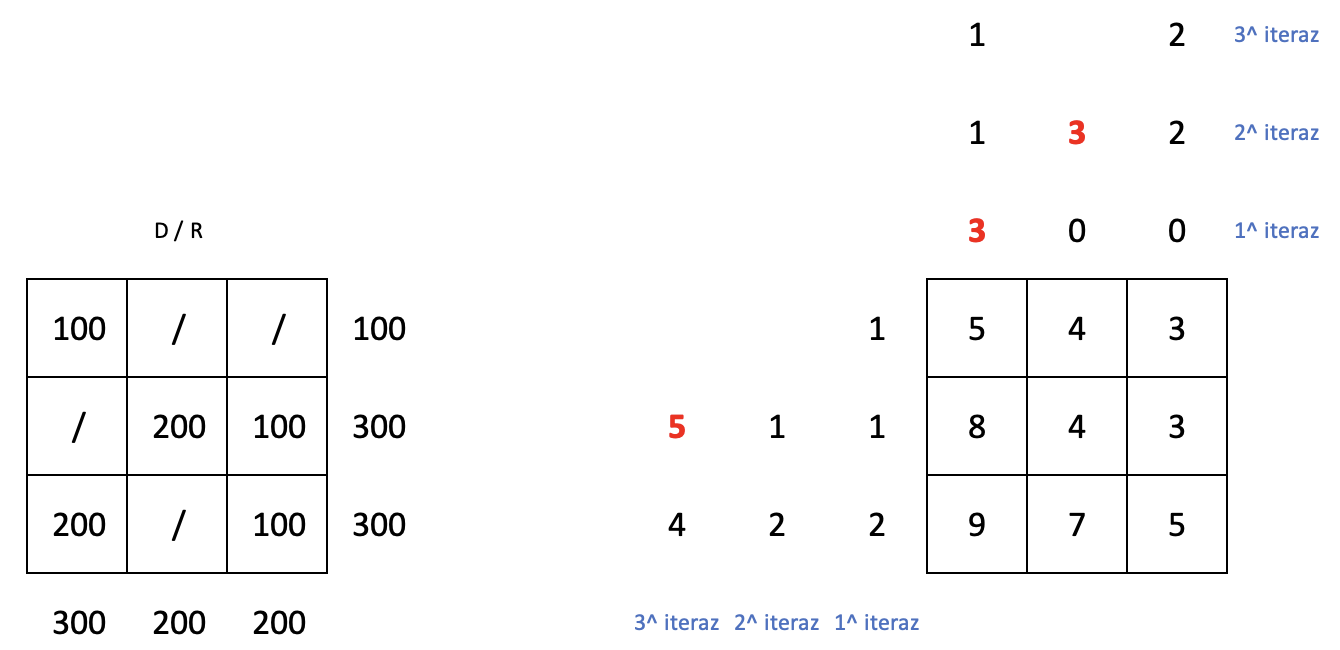
\includegraphics[width=0.4\columnwidth]{img/pb_trasporto_vogel.png}
\end{center}
con un costo pari a $3'900$

\subsection{Metodo Modified Distribution [MODI]}
\'E un metodo che modifica l'algoritmo di stepping stone sfruttando la teoria della dualità. Introduco $R_i, K_j$\\
\\
\textbf{Algoritmo}:
\begin{enumerate}
\item Per ogni cella occupata scrivo: $R_i+K_j = C_{ij}$
\item Scelgo $R_1=0$
\item Per sostituzione ricavo tutte le altre $R_i, K_i$ (a cascata)
\item Definisco $I_{ij}$ per ogni cella vuota, dove $I_{ij} = c_{ij}-R_i-K_j$
\item Seleziono la cella con $I_{ij} < 0$ e più piccolo di tutti gli altri
\item Itero finché trovo tutti gli $I_{ij} >0$ (soluzione ottima)
\end{enumerate}

\subsubsection{Esempio}
Parto con N-W $\rightarrow\ costo = 4'200$
\begin{center}
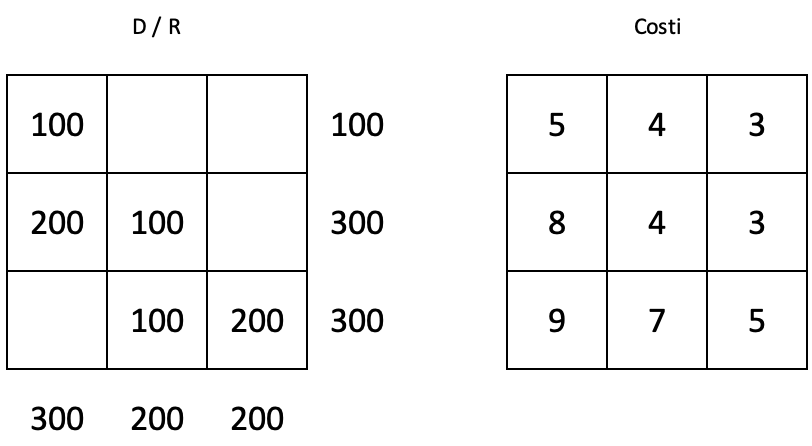
\includegraphics[width=0.4\columnwidth]{img/pb_trasporto_nw.png}
\end{center}
Per applicare MODI vado a calcolarmi gli $R_i$, i $K_j$ e i rispettivi $I_{ij}$:
\begin{enumerate}
\item $\begin{array}{l}R_1+K_1=5\\R_2+K_1=8\\R_2+K_2=4\\R_3+K_2=7\\R_3+K_3=5\end{array}$
\item[2-3.]Pongo $R_1=0 \Rightarrow \begin{array}{l}K_1=5\\R_2=3\\K_2=1\\R_3=6\\K_3=-1 \end{array}$
\item[4.]Mi ricavo gli $I_{ij} \Rightarrow \begin{array}{l}I_{12}=c_{12}-K_1-K_2 = 3\\I_{13}=3-0+1 = 4\\I_{23}=3-3+1 = 1\\I_{31}=9-6-5 = -2\end{array}$
\item[5.] Scelgo l'$I_{ij}$ con valore minore quindi $x_{31}$ va in base
\item[6.] Applico Stepping Stone classico ($min =100$) (MODI serve per scegliere da dove partire) $\rightarrow costo = 4'000$
\end{enumerate}
\begin{center}
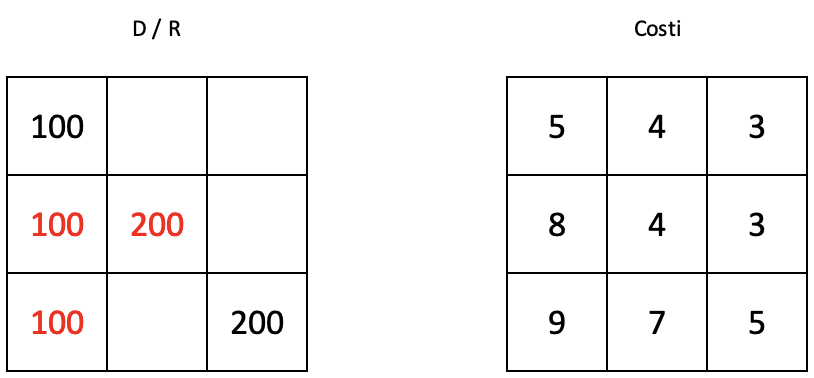
\includegraphics[width=0.4\columnwidth]{img/pb_trasporto_modi.png}
\end{center}
\begin{enumerate}
\item $\begin{array}{l}R_1+K_1=5\\R_2+K_1=8\\R_2+K_2=4\\R_3+K_1=9\\R_3+K_3=5\end{array}$
\item[2-3.]Pongo $R_1=0 \Rightarrow \begin{array}{l}K_1=5\\R_2=3\\K_2=1\\R_3=4\\K_3=1 \end{array}$
\item[4.]Mi ricavo gli $I_{ij} \Rightarrow \begin{array}{l}I_{12}=4-0-1 = 3\\I_{13}=3-0-1 = 2\\I_{23}=3-3-1 = -1\\I_{32}=7-4-1=2 = -2\end{array}$
\item[5.] Scelgo l'$I_{ij}$ con valore minore quindi $x_{23}$ va in base
\item[6.] Applico Stepping Stone classico $\rightarrow costo = 3'900$
\end{enumerate}
\begin{center}
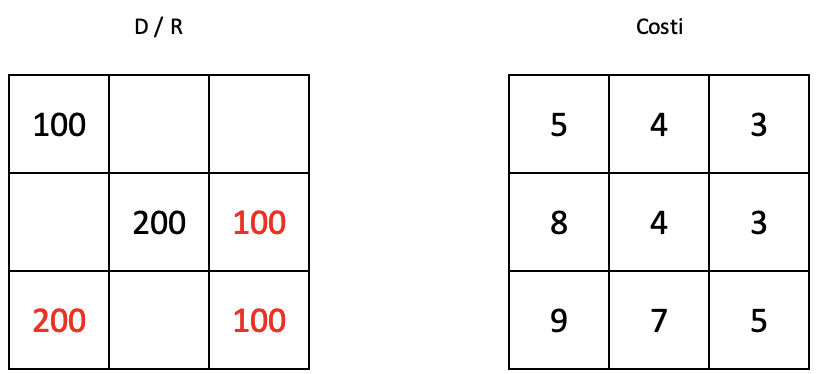
\includegraphics[width=0.4\columnwidth]{img/pb_trasporto_modi2.png}
\end{center}

%CAPITOLO 2
\clearpage
\section{Problema dell'assegnazione}
\begin{center}
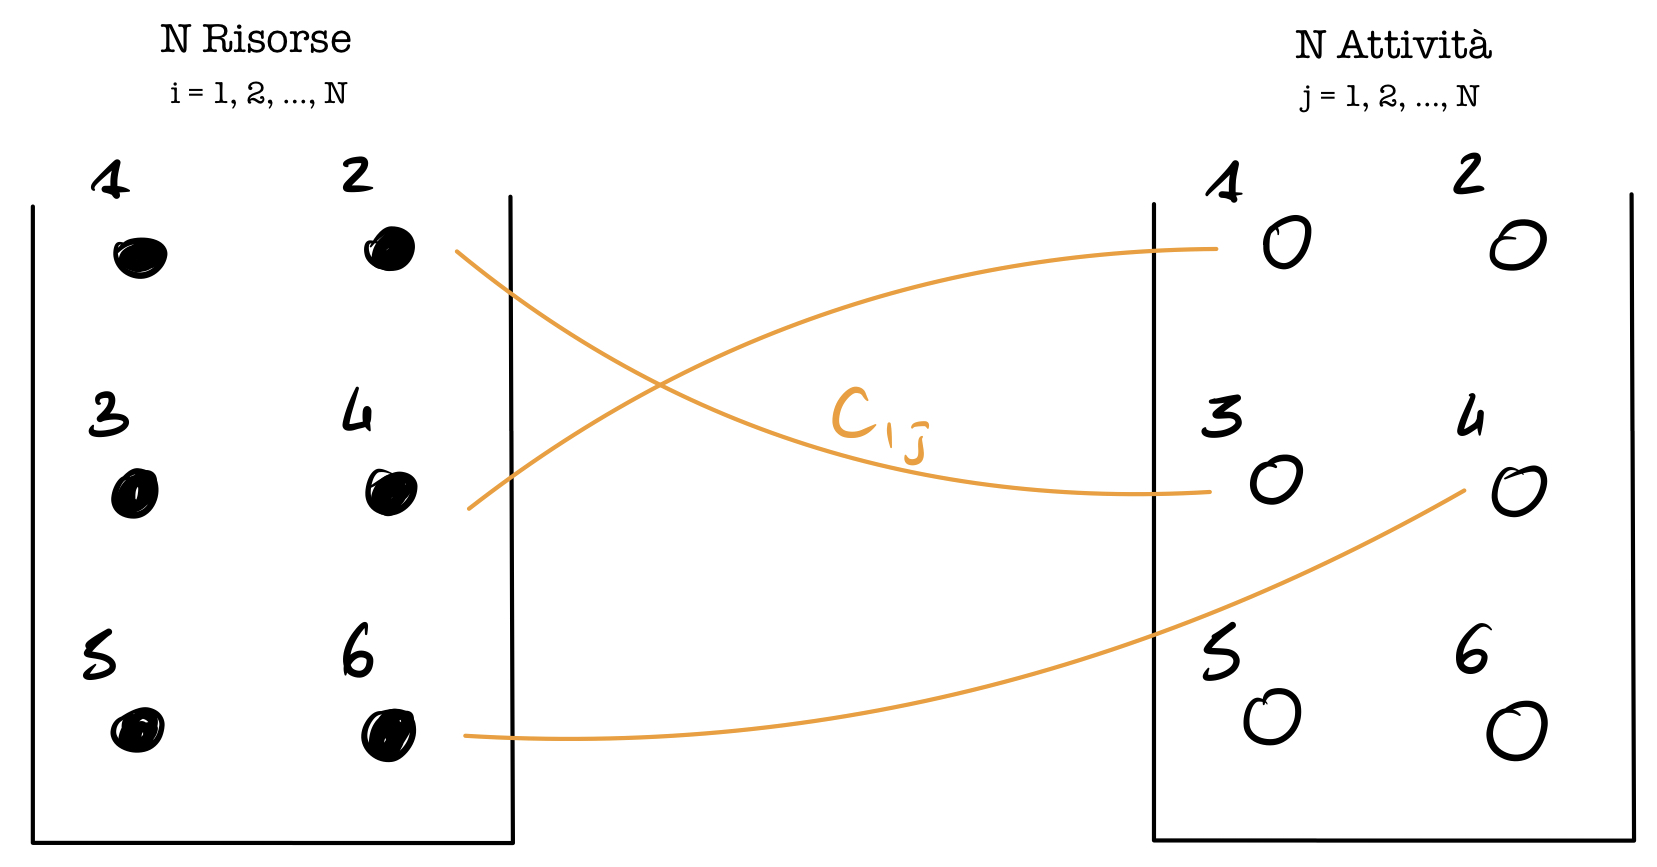
\includegraphics[width=0.4\columnwidth]{img/assegnazione.jpg}
\end{center}

\subsection{Formulazione Matematica}
Problema di programmazione lineare intera [PLI].
\paragraph{Variabili decisionali} $$x_{ij} = \begin{cases}
0 \ \ \ \text{risorsa $i$ non assegnata a attività $j$}\\
1 \ \ \ \text{risorsa $i$ assegnata a attività $j$}\\
\end{cases}•$$
\paragraph{Funzione Obiettivo} $$min\ z = \sum_i^n \sum_j^m x_{ij}\cdot c_{ij}$$
\paragraph{Vincoli} \begin{itemize}
\item $\sum_j x_{ij} = 1, \ \ \forall i = 1, \dots, n$
\item $\sum_i x_{ij} = 1, \ \ \forall j = 1, \dots, n$
\item $x_{ij} \in \{0;1\} \ \ \forall i, j \ \textcolor{red}{\leadsto x_{ij}\geq 0\ \ RILASSATI}$
\end{itemize}

\subsection{Similitudini col problema di trasporto}
$$\begin{array}{l}N=M\\d_i=1 \ \ \forall i\\r_i=1 \ \ \forall j\end{array} \Bigg\}\Rightarrow Assegnazione?$$

\subsection{Parentesi: Rilassamenti di problemi di ottimizzazione}
Siano P e R due problemi:\\
\textbf{P}: $min \ f(x), \ \ x \in F(P)$ dove con F intendo la regione ammissibile (feasable)\\
\textbf{R}: $min \ \phi(x), \ \ x \in F(R)$\\
\\
R è detto rilassamento di P se e solo se:
\begin{enumerate}
\item $F(P) \subseteq F(R)$
\item $\phi(x) \leq (\textcolor{red}{\geq \ se\ di\ massimo})\ f(x), \ \ \forall x \in F(P)$
\end{enumerate}
\begin{center}
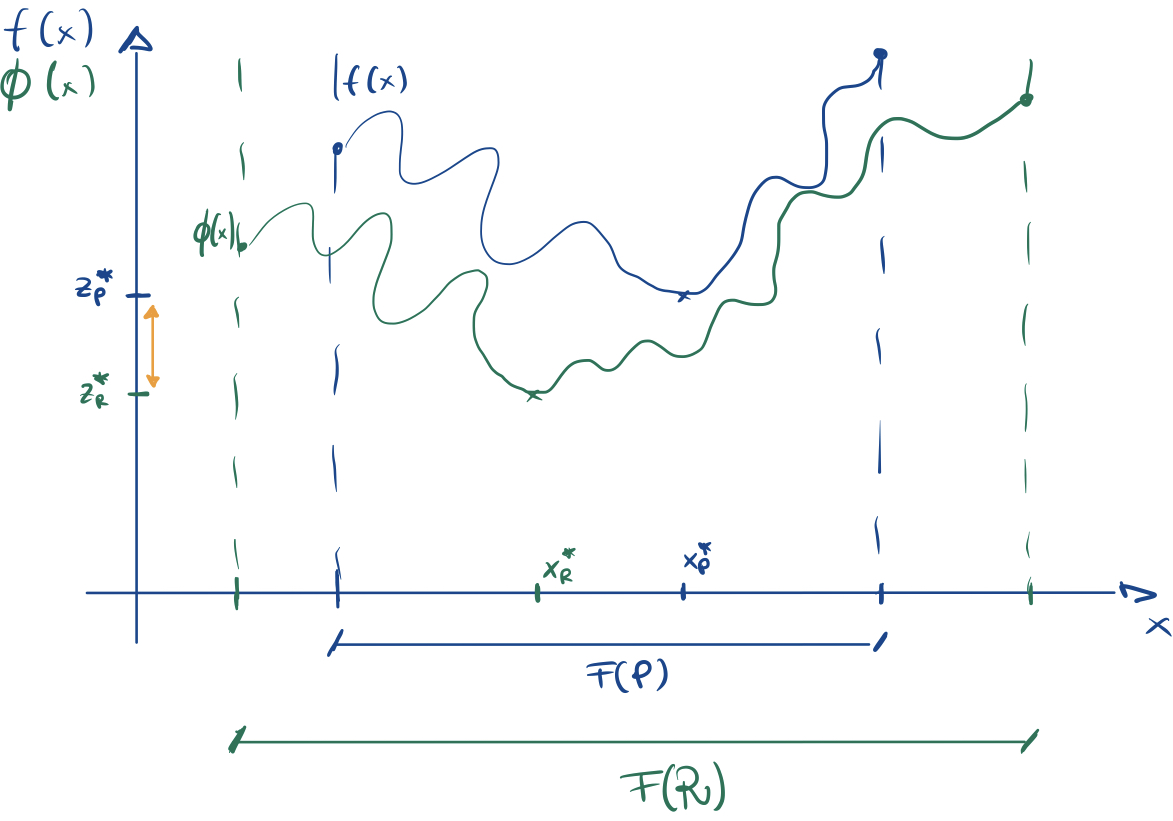
\includegraphics[width=0.5\columnwidth]{img/rilassamento.jpg}
\end{center}

\subsubsection{Quando risolvere un problema rilassato}
\begin{enumerate}
\item R più semplice di P
\item I valori ottimi $z_P^*$ e $z_R^*$ sono prossimi (il più simili possibile)
\item Almeno una soluzione ottima di R dev'essere ammissibile per P
\item Se almeno una soluzione ottima di R è ottima anche per P
\end{enumerate}

\subsubsection{Rilassamento per eliminazione}
Eliminare dei vincoli "alleggerisce" il problema. Si andranno a verificare tali vincoli a posteriori

\subsubsection{Rilassamento lineare (continuo)}
$$\text{Variabili decisionali intere } \leadsto \text{ Variabili decisionali continue}$$
\begin{center}
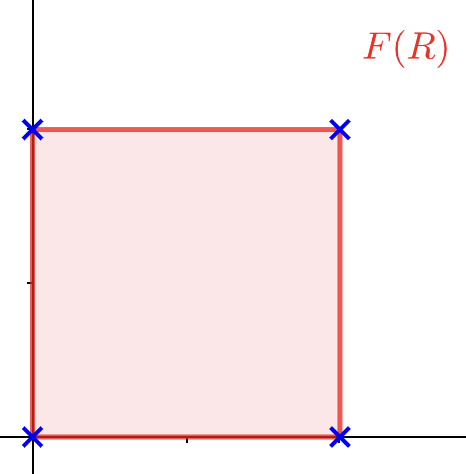
\includegraphics[width=0.3\columnwidth]{img/rilassamento_lineare.png}
\end{center}
\textcolor{blue}{Esempio}: $x_{ij} \in \{0;1\} \leadsto 0\leq x_{ij}\leq 1, \ \ \forall i,j$

\subsubsection{Rilassamento surrogato}
$$max(x=2x_1+3x_2)$$
\begin{equation*}
\begin{cases}
x_1+ x_2 \leq 4\\
2x_1-x_2 \leq 2\\
x_1,x_2 \geq 0
\end{cases} \Rightarrow \begin{cases}
3x_1 \leq 6\\
x_1,x_2 \geq 0
\end{cases}
\end{equation*}
\begin{center}
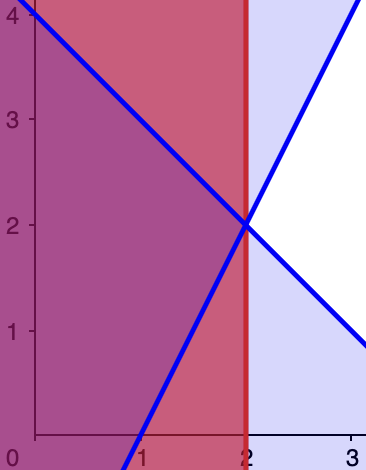
\includegraphics[width=0.3\columnwidth]{img/rilassamento_surrogato.png}
\end{center}

\subsection{Altra parentesi}
\begin{center}
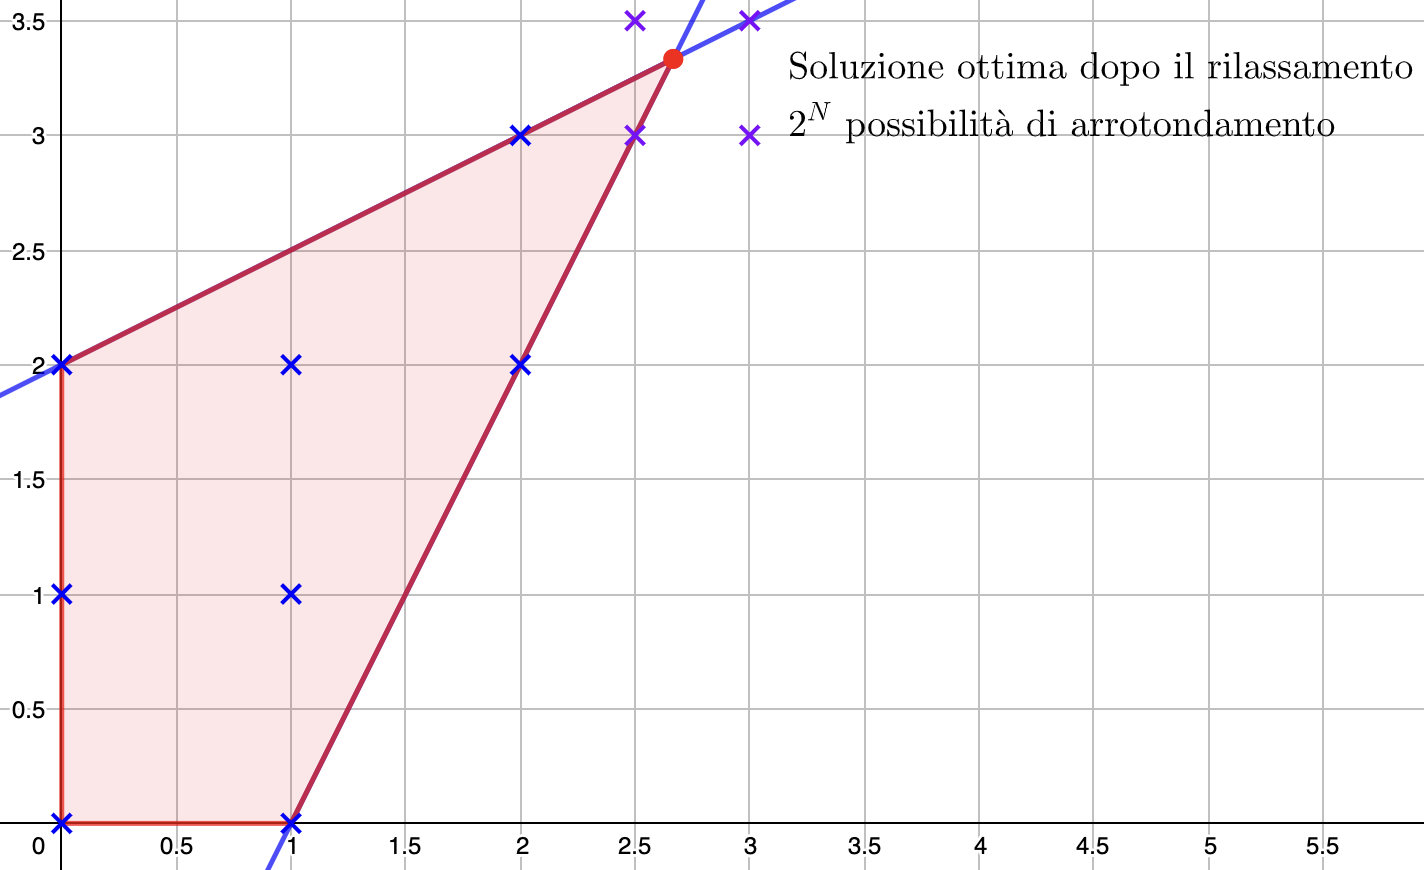
\includegraphics[width=0.4\columnwidth]{img/altra_parentesi.png}
\end{center}

\subsection{Algoritmo ungherese}
Ogni problema di assegnazione ha $N!$ soluzioni ammissibili.
Sia dato il problema con tabella dei costi $c_{ij}$ seguente:
\begin{center}
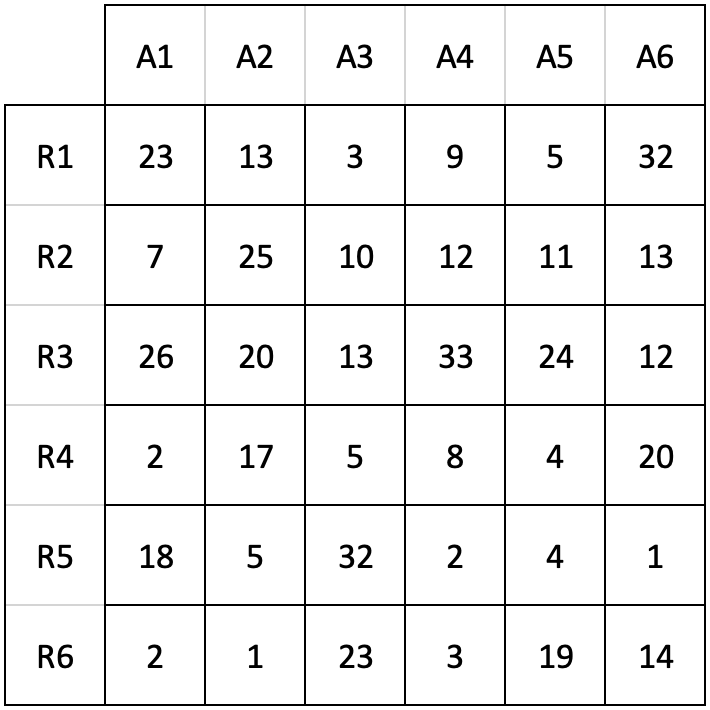
\includegraphics[width=0.4\columnwidth]{img/pb_assegnazione.png}\\
\end{center}

\begin{enumerate}
\item Tolgo il valore minimo ad ogni riga $\textcolor{bluel}{\blacksquare}$
\item Cerco una soluzione a costo 0 $\textcolor{orange}{\blacksquare}$
\item Tolgo il valore minimo ad ogni colonna $\textcolor{gg}{\blacksquare}$
\item Cerco una soluzione a costo 0 $\textcolor{yell}{\blacksquare}$
\begin{center}
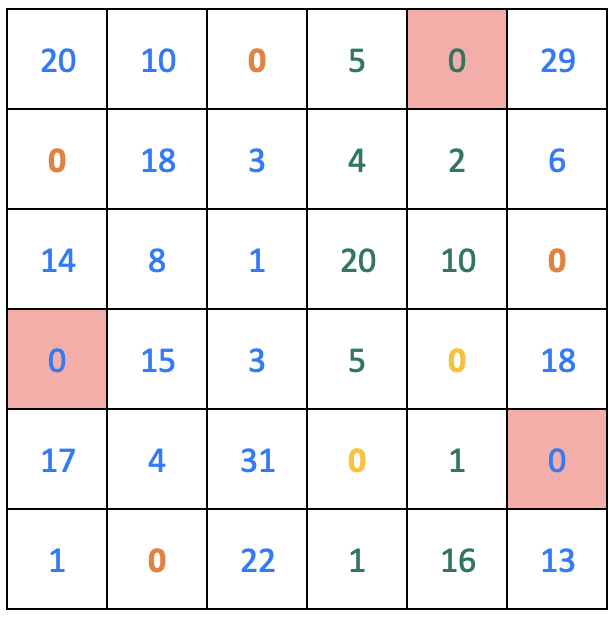
\includegraphics[width=0.4\columnwidth]{img/pb_assegnazione_sol1.png}\\
\end{center}
\clearpage
Caso particolare per procedere con l'algoritmo:\\
Soluzione non ottima, $costo = 86$
\begin{center}
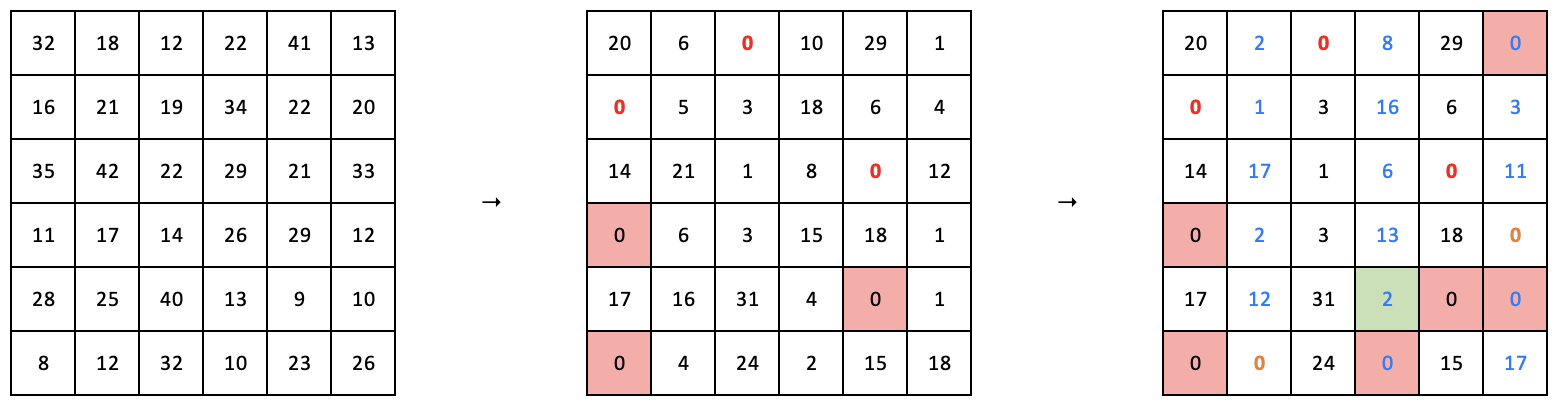
\includegraphics[width=0.9\columnwidth]{img/pb_assegnazione_sol2.png}\\
\end{center}
\item Ricoprimento degli zeri:
\begin{enumerate}
\item Segno le righe senza assegnazione
\item Segno che colonne che hanno "zero" nelle righe segnate
\item Segno le righe che hanno assegnazioni nelle colonne segnate
\item Se al punto 5.c ho aggiunto righe, vai al punto 5.b
\item Le righe coprenti sono le righe non segnate. Le colonne coprenti solo le colonne non segnate: Cinque \emoji{left-arrow}/\emoji{down-arrow} tante quante le assegnazioni obbligate.
\begin{itemize}
\item Trovo un riquadro di "elementi scoperti"
\item Tolgo il valore minimo degli elementi scoperti e lo sottraggo a tutti gli elementi scoperti
\item Sommo tale valore delle righe/colonne dove c'è sovrapposizione
\end{itemize}
\end{enumerate}
\end{enumerate}
\begin{center}
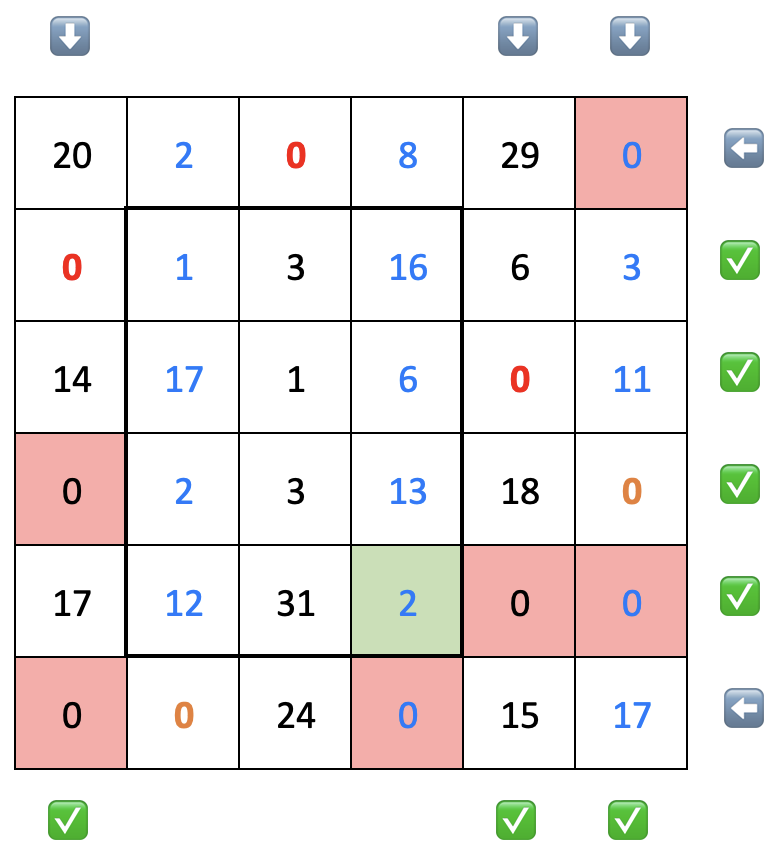
\includegraphics[width=0.3\columnwidth]{img/pb_assegnazione_sol3.png}\\
\end{center}
Ottenendo così un $costo=85$, che nel nostro caso è una soluzione ottima.
\begin{center}
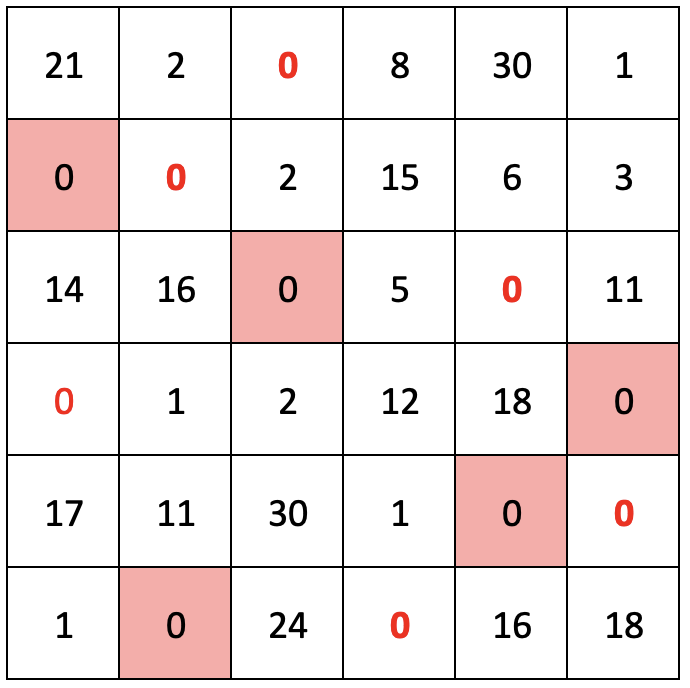
\includegraphics[width=0.3\columnwidth]{img/pb_assegnazione_sol4.png}\\
\end{center}
E qualora avessi un problema di massimizzazione? [Non è un problema di assegnazione!]\\
Vado a considerare $p_{ij}$ profitti
$$max\ z = \sum_i \sum_j p_{ij}\cdot x_{ij} \ \ \ \ 0 \leq p_{ij} \leq \hat p_{\bar i \bar j} = max_{ij}\{p_{ij}\}$$
$\rightarrow$ costruisco un problema di assegnazione:\\
Pongo $c_{ij} := \hat p_{\bar i \bar j} - p_{ij}, \forall i,j$ (complemento dei profitti rispetto al profitto massimo)\\
$z' = \sum_i \sum_j (\hat p_{\bar i \bar j} - p_{ij})x_{ij} = \sum_i\sum_j \hat p_{\bar i \bar j}\cdot x_{ij} - \sum_i \sum_j p_{ij}\cdot x_{ij} = min\ \alpha = max\ (-\alpha) \rightarrow min\ z' = max\ z$\\
\\
\textcolor{blue}{Esempio}:
\begin{center}
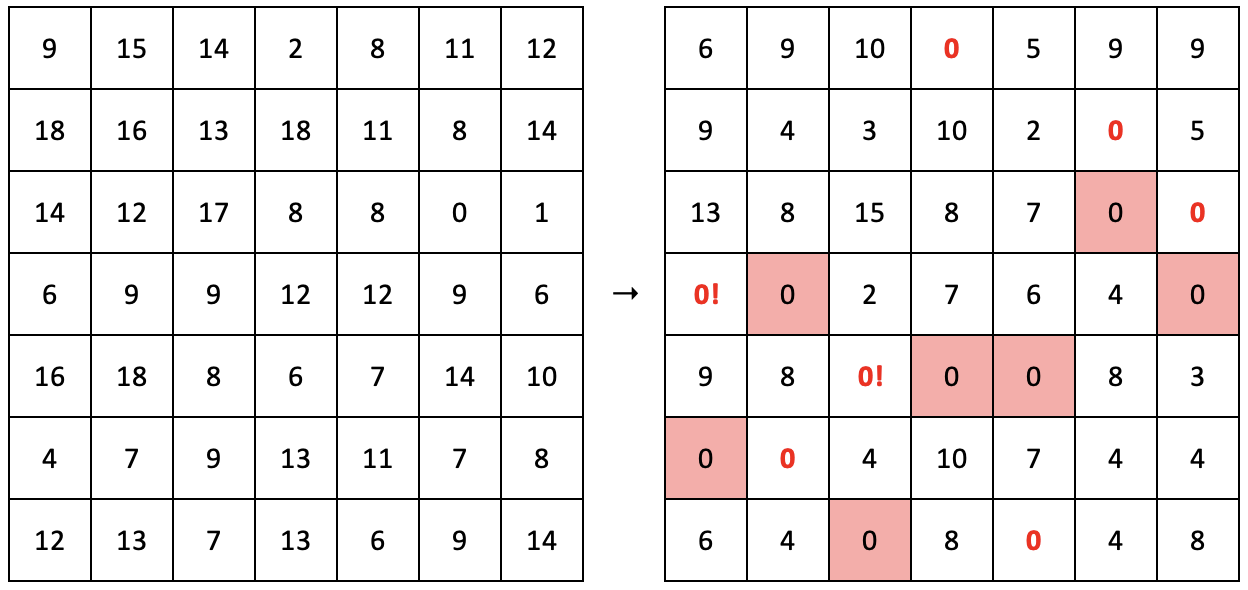
\includegraphics[width=0.5\columnwidth]{img/esempio_pb_assegnazione.png}\\
\end{center}
Dove ho messo dei \textbf{\textcolor{red}{!}} vuol dire che ho fatto delle scelte. Le soluzioni ottime possibili sono $2^k$, dove $k=\#$ scelte (non obbligate) fatte\\
\\
Più nello specifico:
\begin{itemize}
\item Stallo dopo il $\textcolor{red}{\blacksquare}$, non ho più scelte obbligate
\item Inizio a operare in maniera arbitraria $\textcolor{orange}{\blacksquare}$
\item Continuando vedo se sono obbligato in delle scelte $\textcolor{bluel}{\blacksquare}$
\end{itemize}
\begin{center}
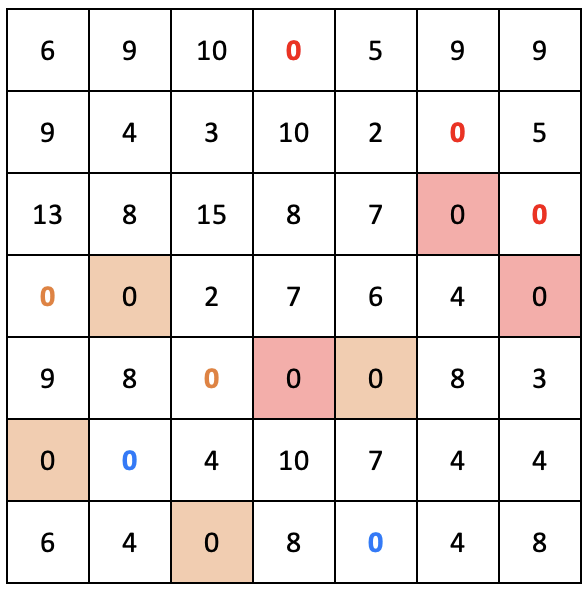
\includegraphics[width=0.3\columnwidth]{img/stallo_pb_assegnazione.png}\\
\end{center}
\textcolor{blue}{Caso ancora più patologico}\\
Le soluzioni ottime sono tante quante le soluzioni ammissibili $\Rightarrow \ 4!$\\
\\
$\textcolor{blue}{\blacksquare} \rightarrow arbitraria$\\
$\textcolor{red}{\blacksquare} \rightarrow obbligata$
\begin{center}
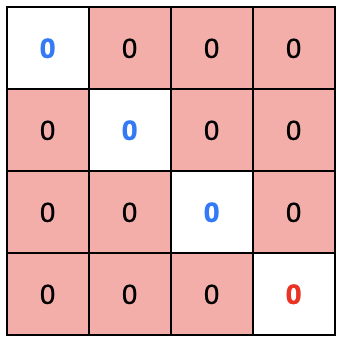
\includegraphics[width=0.3\columnwidth]{img/caso_patologico_assegnazione.png}\\
\end{center}

%CAPITOLO 3
\clearpage	
\section{Problema del flusso massimo [MAX FLOW]}
\begin{center}
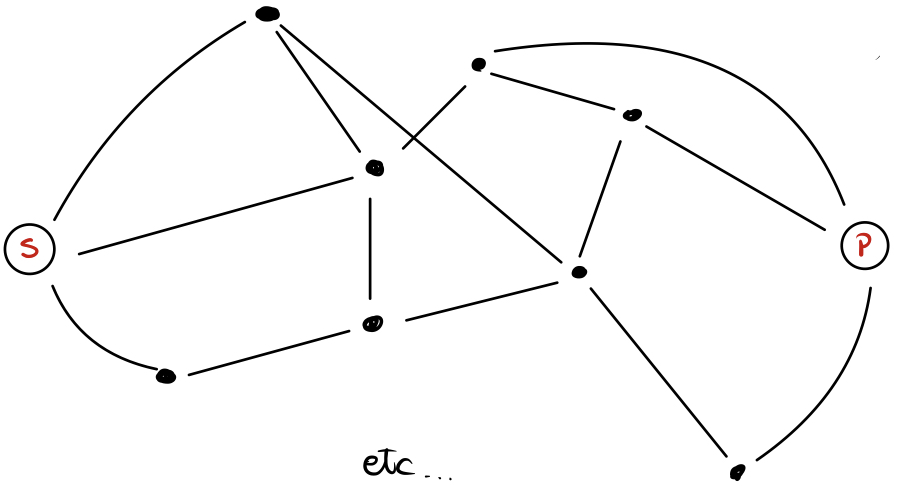
\includegraphics[width=0.6\columnwidth]{img/max_flow.jpeg}\\
\end{center}
\subsection{Formulazione Matematica}
ll problema del flusso massimo viene descritto dalla funzione $G=(\aleph,\ A)$ dove $$\begin{array}{ll}\aleph & \text{insieme dei nodi}\\A & \text{insieme degli archi (orientati)}\end{array}$$
\paragraph{Variabili decisionali}: $$x_{ij} =  \text{ quantità del flusso lungo l'arco } (i,j) \in A$$
\paragraph{Funzione obiettivo}: $$max \ z = \sum_{(S,j)\in \delta^+(S)}x_{S,j} - \sum{(i,S)\in \delta^-(S)}x_{i,S}$$
\textbf{Nota Bene}: $\delta^+(S)$ e $\delta^-(S)$ mi rappresentano gli insiemi di archi uscenti ed entranti nel punto S. Nell'esempio seguente: $\begin{array}{l}\delta^+ (S)= \{(S,a);(S,b)\}\\\delta^-(S) = \{(c,S)\}\end{array}$
\begin{center}
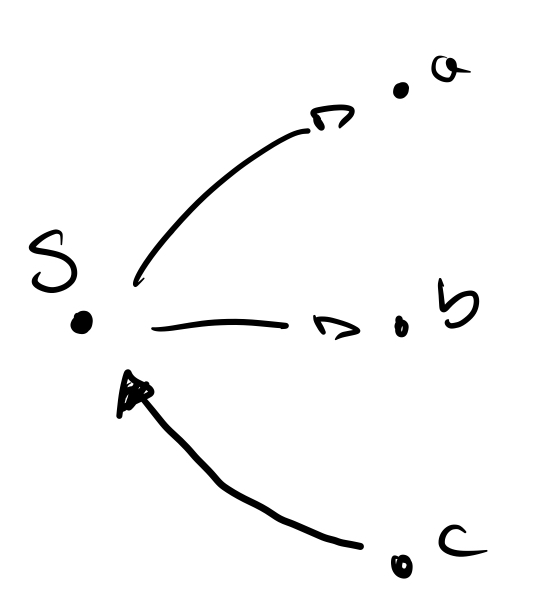
\includegraphics[width=0.3\columnwidth]{img/archi_es.jpeg}\\
\end{center}
\paragraph{Vincoli}
$$\sum_{(i,j)\in \delta^+(i)}x_{ij} - \sum_{(i,j)\in \delta^-(i)} = 0, \ \ \forall i, \in \aleph \setminus\{S;P\}$$
$$0 \leq x_{ij} \leq u_{ij}, \ \ \forall (i,j) \in A$$
Condizione sui dati: $u_{ij} \geq 0, \ \forall (i,j) \in A$

\subsection{Vediamo un istanza}
\begin{center}
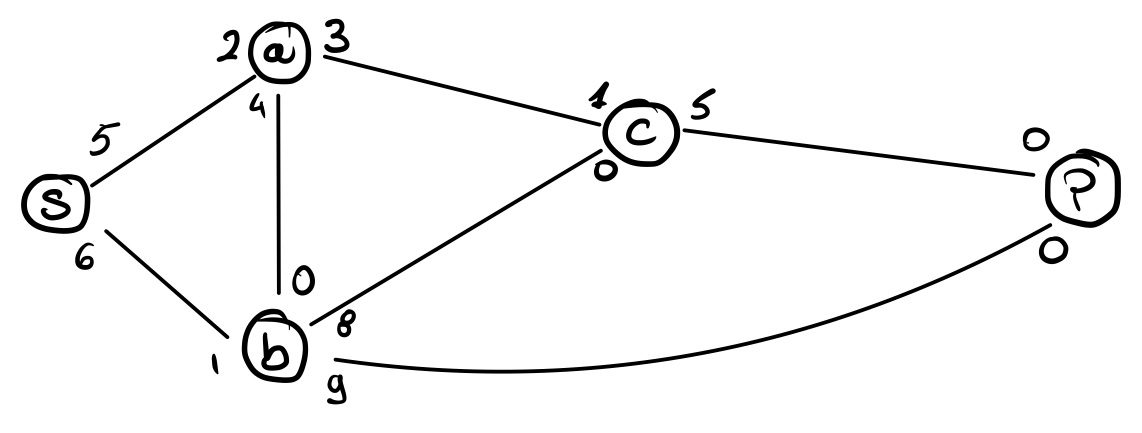
\includegraphics[width=0.6\columnwidth]{img/pb_maxflow_es.jpg}\\
\end{center}
{\scriptsize\textcolor{blue}{\textbf{Nota Notazionale}:} \begin{center}
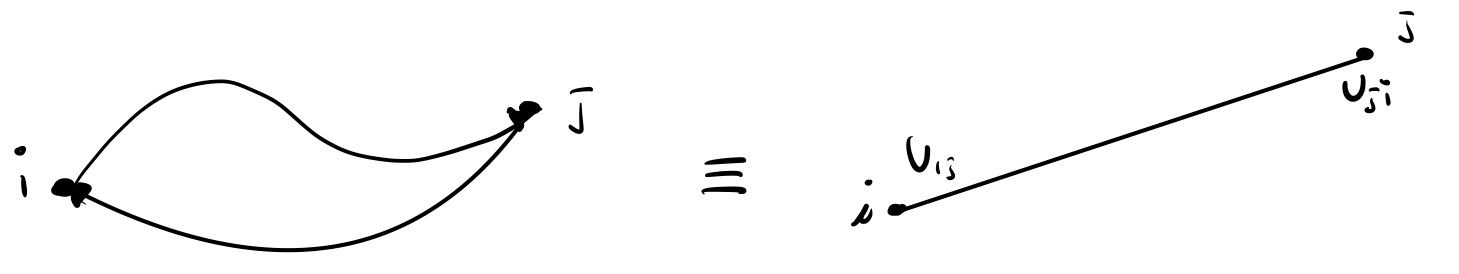
\includegraphics[width=0.5\columnwidth]{img/pb_maxflow_nota.jpeg}\\
\end{center}}
$\aleph = \{S,\ a,\ b,\ c,\ P\}; \ \ \ A = \{(S,a), (S,b),(a,S),(a,b),(b,S),(a,c),(b,a), (c,a), (b,c),(b,P),$\\$(c,b),(P,b),(c,P), (P,c)\}$\\
Vincoli:
\begin{enumerate}
\item[a)] $x_{Sa} + x_{ba}+x_{ca}-x_{aS} - x_{ab}-x_{ac}$
\item[b)] $x_{Sb} + x_{ab}+x_{cb}+x_{Pb}-x_{bS} - x_{ba}-x_{bc}-x_{bP}$
\item[c)] $x_{ac} + x_{bc}+x_{Pc}-x_{ca} - x_{cb}-x_{cP}$
\end{enumerate}
$\begin{array}{cc}
0 \leq x_{Sa} \leq 5 & 0 \leq x_{as} \leq 2\\
0 \leq x_{Sb} \leq 6 & 0 \leq x_{bs} \leq 1\\
0 \leq x_{ab} \leq 4 & 0 \leq x_{ba} \leq 0\\
0 \leq x_{ac} \leq 3 & 0 \leq x_{ca} \leq 1\\
0 \leq x_{bc} \leq 8 & 0 \leq x_{cb} \leq 0\\
0 \leq x_{bP} \leq 5 & 0 \leq x_{Pb} \leq 0\\
0 \leq x_{cP} \leq 9 & 0 \leq x_{Pc} \leq 0\\
\end{array}$

\subsection{Algoritmo di Ford - Fulkerson}
\begin{enumerate}
\item Individuo un cammino: $S-a-c-P: 3$ (trasporto tre perché è il collo di bottiglia del percorso)
\item Aggiorno le capacità in entrambi i sensi $\textcolor{red}{\blacksquare}$
\begin{center}
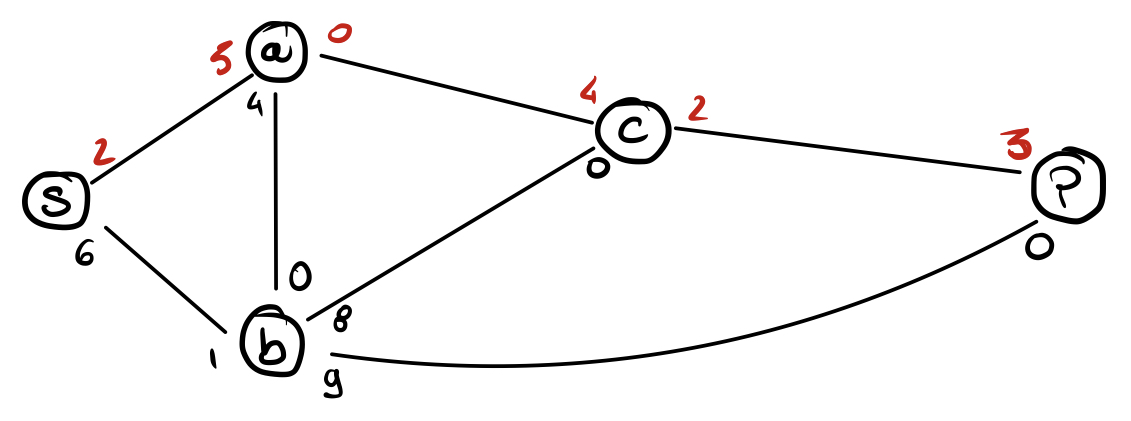
\includegraphics[width=0.4\columnwidth]{img/max_flow_ff1.jpeg}\\
\end{center}
\item Trovo un cammino aumentante
\item Vai al punto 2
\end{enumerate}
Dopo un paio di passaggi, nella nostra istanza, arrivo a un flusso risultante di $11$ trovando due percorsi aumentanti $S-a-b-c-P:2\ \ \textcolor{bluel}{\blacksquare}$ e $S-b-P:6\ \ \textcolor{gg}{\blacksquare}$
\begin{center}
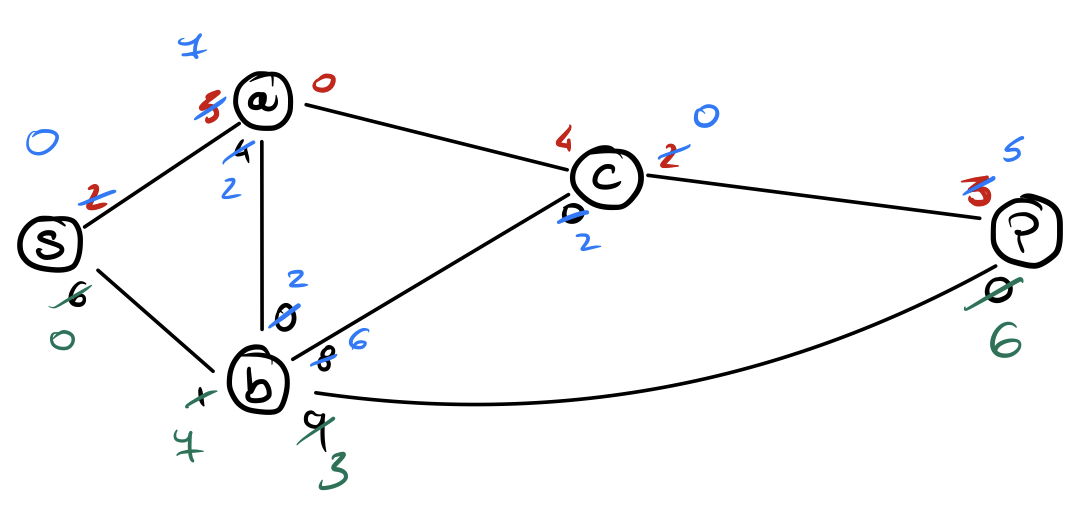
\includegraphics[width=0.4\columnwidth]{img/max_flow_ff2.jpeg}\\
\end{center}

\subsection{Istanza più complicata}
\begin{center}
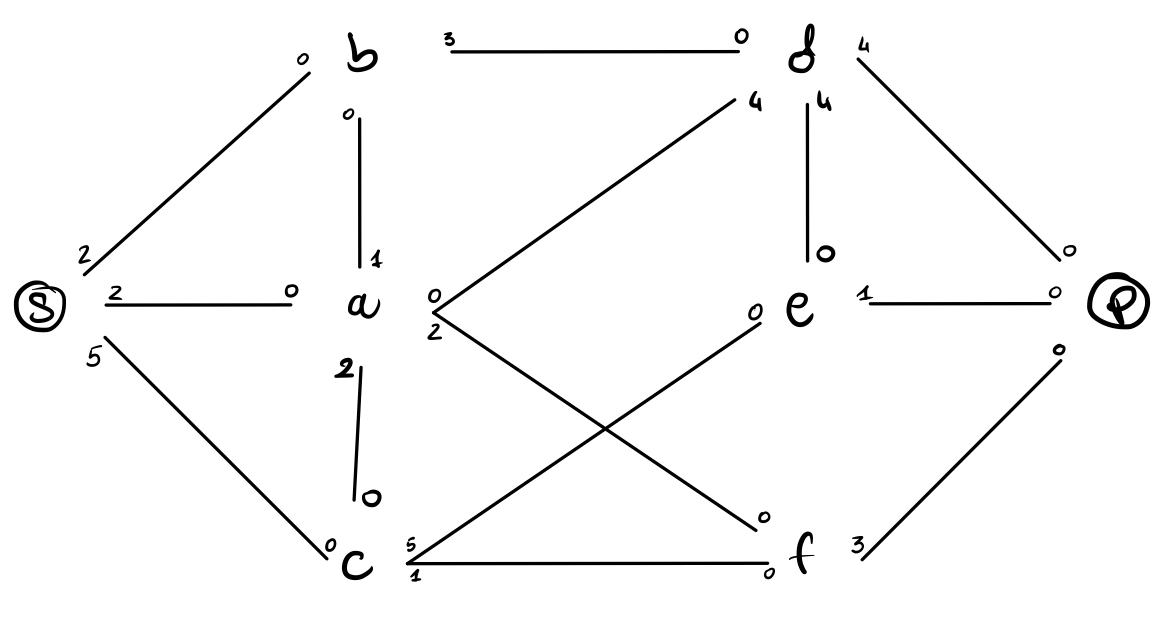
\includegraphics[width=0.4\columnwidth]{img/pb_maxflow_es.jpeg}\\
\end{center}
Cammino: $S-b-d-P: 2 \ \ \textcolor{red}{\blacksquare}; \ \ S-a-b-d-P: 1 \ \ \textcolor{bluel}{\blacksquare}; \ \ S-a-f-P: 1 \ \ \textcolor{gg}{\blacksquare}; \ \ S-c-e-P: 1 \ \ \textcolor{or}{\blacksquare}; \ \ S-c-f-P: 2 \ \ \textcolor{pp}{\blacksquare}$
\begin{center}
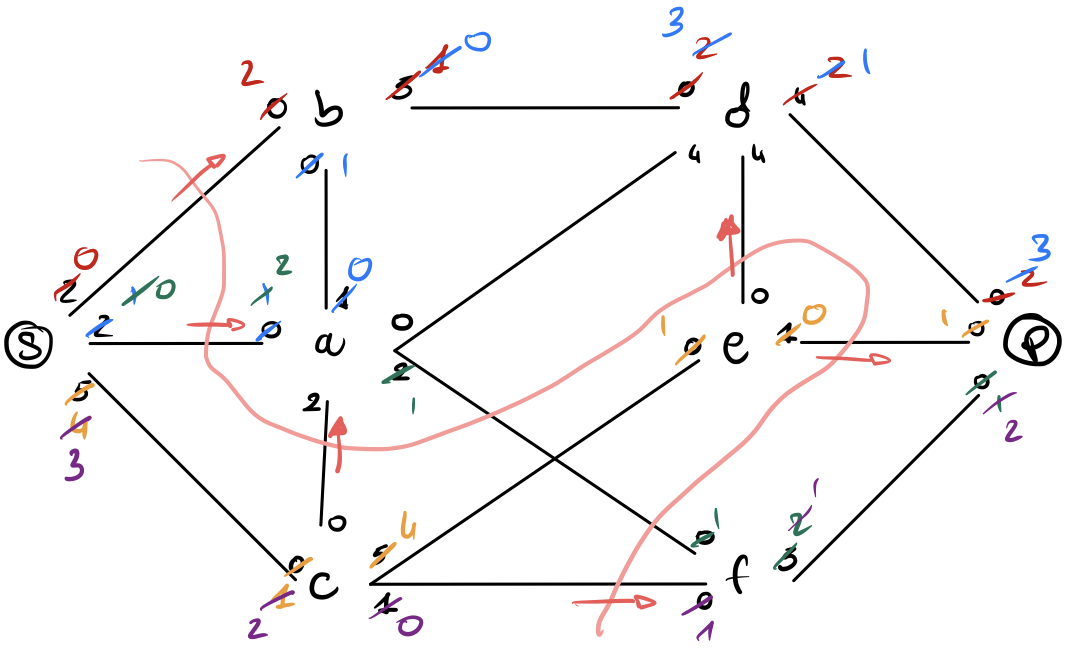
\includegraphics[width=0.4\columnwidth]{img/pb_maxflow_esc.jpeg}\\
\end{center}
La riga $\textcolor{rose}{\blacksquare}$ mi rappresenta il taglio S-P dell'istanza e $\textcolor{rose2}{\rightarrow}$ gli archi tagliati.\\
\\
\textcolor{blue}{\textbf{Definizione} [Taglio S-P in una rete]:}
$$\begin{array}{ccc}
\aleph = \aleph_1 \cup \aleph_2 & e &\aleph_1 \cap \aleph_2 = \emptyset\\
S \in \aleph_1 & e & P \in \aleph_2
\end{array}$$
\textcolor{blue}{\textbf{Definizione} [Flusso attraverso il taglio S-P]:}
$$\sum_{(i,j)\in \delta^+(\aleph_1)}x_{ij} - \sum_{(i,j)\in \delta^-(\aleph_1)} x_{ji}$$
\textcolor{blue}{\textbf{Definizione} [Capacità del taglio S-P]:}
$$\sum_{(i,j)\in \delta^+(\aleph_1)}u_{ij}$$

\subsection{Istanza patologica}
\begin{center}
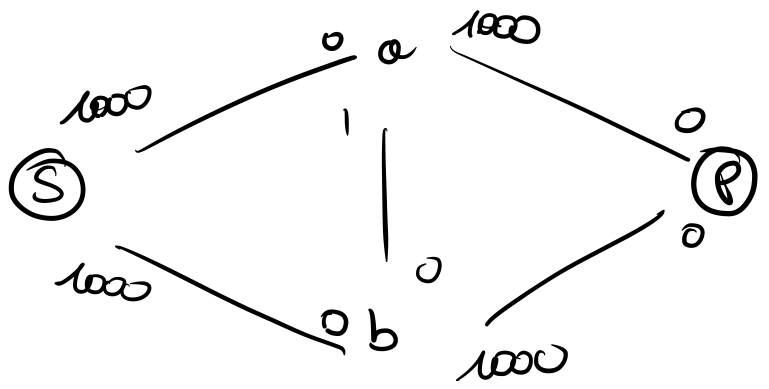
\includegraphics[width=0.5\columnwidth]{img/pb_maxflow_pat.jpeg}\\
\end{center}
Poterebbe capitare un istanza dove prendendo dei specifici cammini $S-a-b-P: 1 \ \ \textcolor{red}{\blacksquare}; \ S-b-a-P: 1 \ \ \textcolor{bluel}{\blacksquare}$ ci si impiegherebbero un sacco di passaggi inutili.
\begin{center}
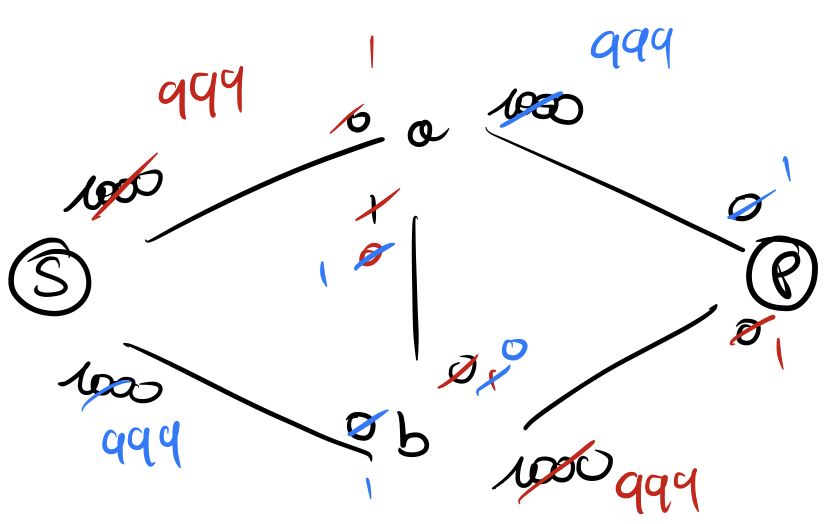
\includegraphics[width=0.4\columnwidth]{img/pb_maxflow_patsol.jpeg}\\
\end{center}
Per questo motivo nell'algoritmo può essere introdotta la \textbf{regola di Edmonds \& Karp} ossia quella di preferire i cammini con meno archi coinvolti

\subsection{Problemino}
\textbf{Specifiche}:\\
$P_1$ deve essere completati entro i prossimi $3\ mesi$\\
$P_2$ deve essere completati entro i prossimi $4\ mesi$\\
$P_3$ deve essere completati entro i prossimi $2\ mesi$\\
\\
$P_1$ impiega una forza di lavoro pari a $8\ mesi \times uomo$\\
$P_2$ impiega una forza di lavoro pari a $10\ mesi \times uomo$\\
$P_3$ impiega una forza di lavoro pari a $12\ mesi \times uomo$\\
\\
Non si possono utilizzare più di $8\ risorse$ in un mese e possono lavorare allo stesso progetto un massimo di $6\ persone$ in un certo mese.\\
\\
\textbf{Risoluzione}:
Imposto il problema come un problema di flusso massimo
\begin{center}
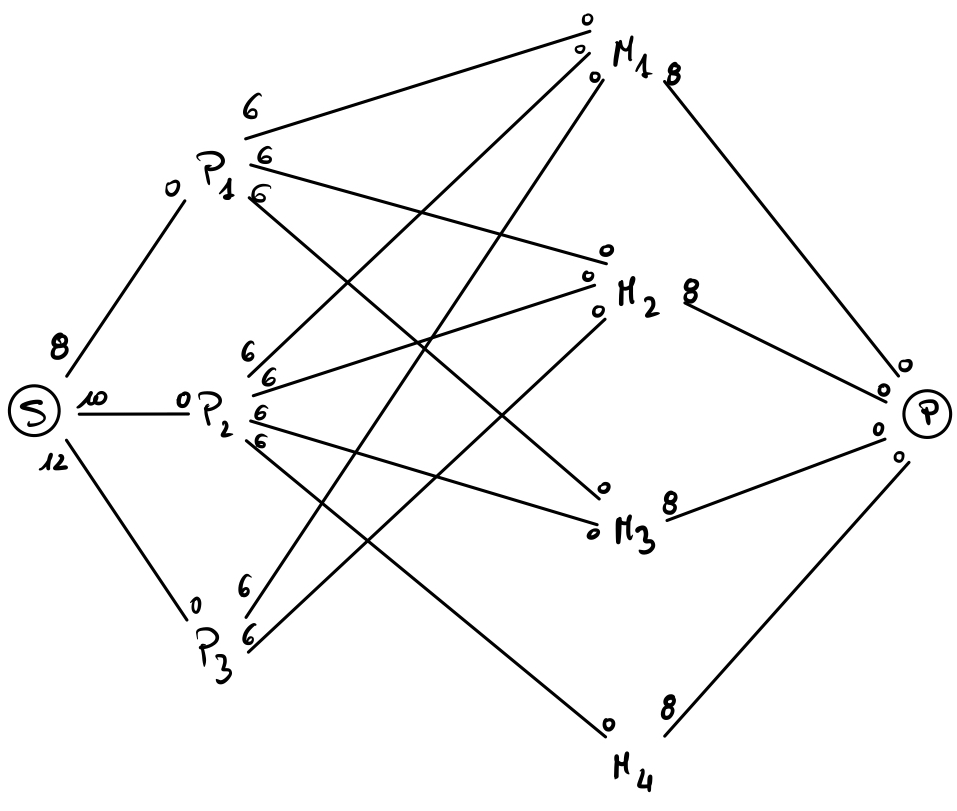
\includegraphics[width=0.4\columnwidth]{img/pb_maxflow_problemino.jpg}\\
\end{center}
Inizio coi cammini: $S-P_1-M_1-P: 6 \ \ \textcolor{red}{\blacksquare}; \ \ S-P_2-M_2-P: 6 \ \ \textcolor{bluel}{\blacksquare}; \ \ S-P_3-M_1-P: 2 \ \ \textcolor{or}{\blacksquare}; \ \ S-P_1-M_2-P: 2 \ \ \textcolor{gg}{\blacksquare}; \ \ S-P_2-M_3-P: 4 \ \ \textcolor{rose}{\blacksquare};\ \ S-P_3-M_1-P_1-M_3-P: 4 \ \ \textcolor{pp}{\blacksquare}; \ \ S-P_3-M_2-P_2-M_4-P: 6 \ \ \textcolor{gg2}{\blacksquare}$\\
\begin{center}
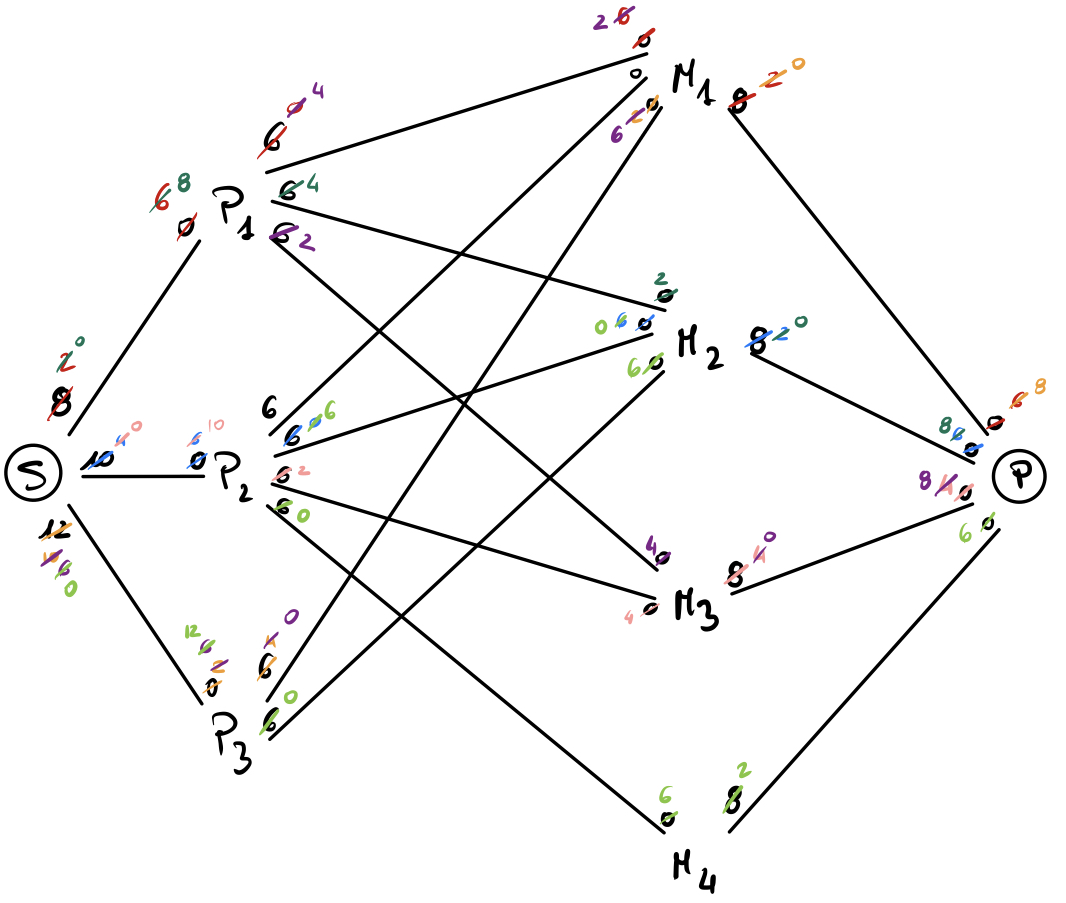
\includegraphics[width=0.5\columnwidth]{img/pb_maxflow_problemino_sol.jpg}\\
\end{center}
$\aleph_1=\{S\}, \ \ \aleph_2 = \aleph \setminus \aleph_1$\\
\textbf{Soluzione}:
\begin{center}
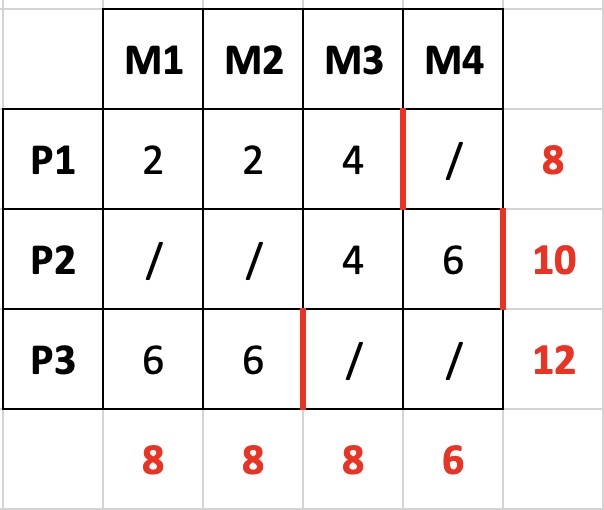
\includegraphics[width=0.4\columnwidth]{img/pb_maxflow_problemino_tab.JPG}\\
\end{center}

%CAPITOLO 4
\clearpage
\section{Problema del cammino minimo [SPP]}
\textbf{SPP}: Shortest Path Problem
\begin{center}
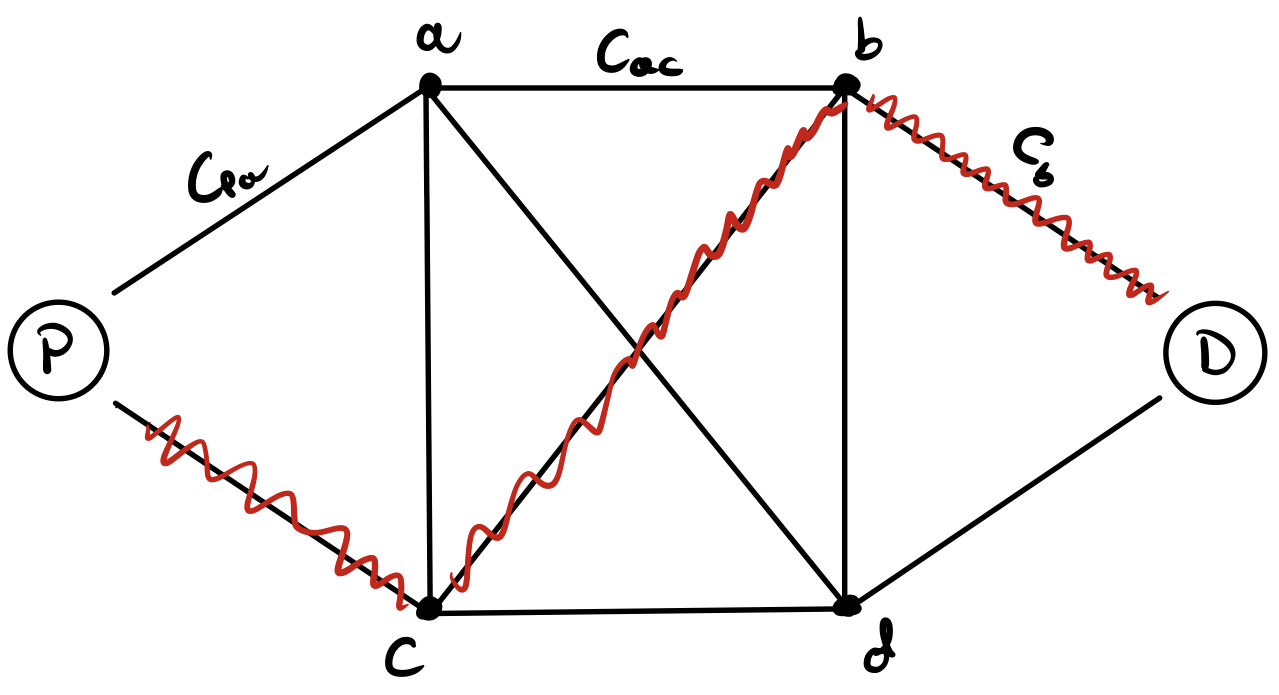
\includegraphics[width=0.6\columnwidth]{img/spp.jpeg}\\
\end{center}
$\textcolor{red}{\blacksquare}$: Soluzione indicativa
\subsection{Formulazione Matematica}
ll problema del cammino minimo è un problema su reti e viene descritto dalla funzione $G=(\aleph,\ A)$ dove $$\begin{array}{ll}\aleph & \text{insieme dei nodi}\\A & \text{insieme degli archi (orientati)}\end{array}$$
$c_{ij}$ mi rappresentano quelli che sono i costi di percorrenza degli archi.
\paragraph{Variabili decisionali} $$x_{ij} = \begin{cases}
0 \ \ \ \text{se $(i,j)\not \in$ percorso a costo minimo}\\
1 \ \ \ \text{se $(i,j) \in$ percorso a costo minimo}\\
\end{cases}$$
\paragraph{Funzione Obiettivo} $$min\ z = \sum_i^n \sum_j^m x_{ij}\cdot c_{ij}$$
\paragraph{Vincoli}
\begin{enumerate}
\item[P)] $$\sum_{(P,j) \in \delta^+(P)} x_{Pj}=1$$
\item[D)] $$\sum_{(i,D) \in \delta^-(D)} x_{iD}=1$$
\end{enumerate}
\textbf{Altri vincoli funzionali}: $$\sum_{(h,j) \in \delta^+(h)} x_{hj} - \sum_{(i,h) \in \delta^-(h)} x_{ih}=0 \ \ \ \forall h \in \aleph \setminus \{P;\ D\}$$
\textbf{Vincoli di dominio}: $x_{ij} \in \{0;1\}; \ \ \forall (i,j) \in A$\\
\textbf{Condizione sui parametri}: $c_{ij} \geq 0,\ \ \forall (i,j) \in A$

\subsection{Algoritmo risolutivo [Dijkstra]}
\begin{enumerate}
\item \textbf{Inizializzazione}
\begin{itemize}
\item $d[P]=0$ distanza nodo iniziale = 0
\item $d[i]=\infty$ distanza iniziale di ogni nodo diverso da P
\item $pred[i] = i$ ogni nodo ha predecessore se stesso
\item $L = \{P\}$ la lista dei nodi da analizzare contiene il nodo P
\item $S=\{\}$ la lista dei nodi già analizzati/etichettati
\end{itemize}
\item \textbf{Iterazione}\\
Finché la lista dei nodi da visitare $L$ non è vuota:
\begin{itemize}
\item Estrarre dalla lista $L$ il nodo $x$ con distanza più bassa
\item Eliminare il nodo $x$ dalla lista $L$ (nodi da analizzare)
\item Aggiungere il nodo $x$ alla lista $S$ (nodi analizzati)
\item Analizzare ogni nodo $j$ adiacente di $x$ se $j$ non è in $S$ (nodi analizzati)
\begin{itemize}
\item Calcolare la distanza dei nodi adiacenti del nodo $x \ d'[j] = d[x] + c(x,j)$
\item Se ll costo $d'[j]<d[j]$
\begin{itemize}
\item Aggiornare il vettore $d[j]=d'[j]$
\item Aggiornare il predecessore $pred[j]=x$
\item Aggiungere alla lista $L$ il nodo adiacente $j$ (se non presente)
\end{itemize}
\end{itemize}
\end{itemize}
Al termine dell'esecuzione l'algoritmo indica il costo minimo $d[i]$ del percorso per raggiungere l'i-esimo nodo a partire dal nodo iniziale $P$.\\Se un valore $d[i]$ è infinito, vuol dire che l'i-esimo nodo non è raggiungibile da $P$.
\end{enumerate}
\url{https://it.wikipedia.org/wiki/Algoritmo_di_Dijkstra}

\subsection{Esempio}
\begin{center}
\begin{tabular}{l c l}
\parbox{0.4\columnwidth}{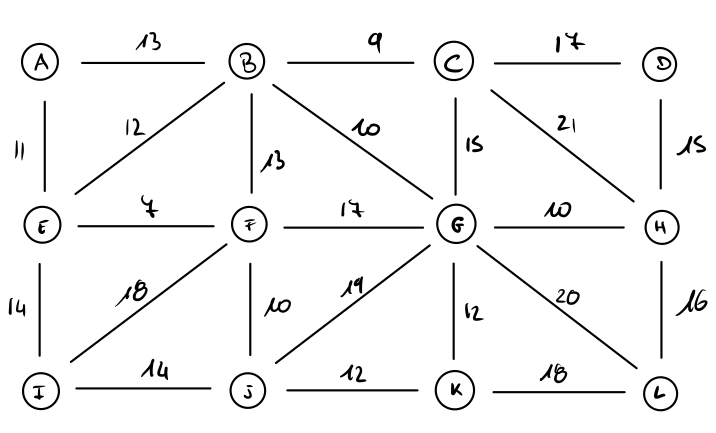
\includegraphics[width=0.4\columnwidth]{img/spp_es.jpg}} &
\parbox{0.05\columnwidth}{$\longrightarrow$} & \parbox{0.4\columnwidth}{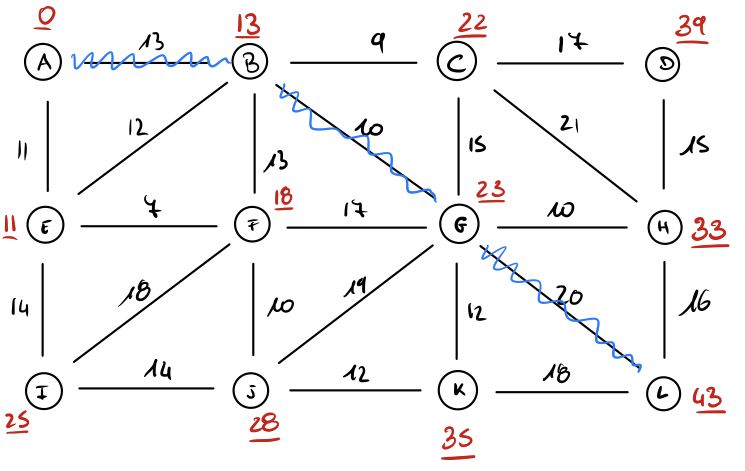
\includegraphics[width=0.4\columnwidth]{img/spp_es_sol.jpg}}\\
\end{tabular}
\end{center}


%CAPITOLO 5
\clearpage
\section{Alberi Minimi}
\subsection{Richiamo \& Definizioni}
\textbf{Archi adiacenti}: Archi che condividono un nodo
\begin{center}
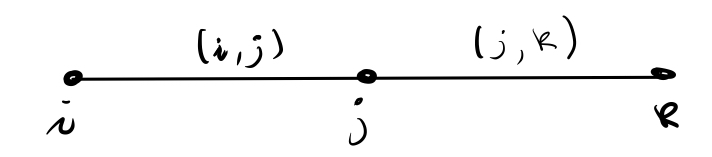
\includegraphics[width=0.4\columnwidth]{img/arch_adiac.jpg}\\
\end{center}
\textbf{Cammino / Percorso}: Sequenza di archi a due a due adiacenti
\begin{center}
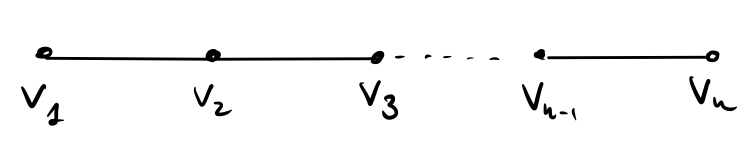
\includegraphics[width=0.4\columnwidth]{img/cammino.jpg}\\
\end{center}
\textbf{Cammino semplice}: Cammino che non contiene cicli
\begin{center}
\includegraphics[width=0.4\columnwidth]{img/camm_sempl.jpg}\\
\end{center}
\textbf{Ciclo / Circuito}: Cammino con $v_1=v_n$\\
\textbf{Grafo Connesso}: Esiste (almeno) un cammino per ogni coppia possibile di nodi
\begin{center}
\includegraphics[width=0.4\columnwidth]{img/grafo_conn.jpg}\\
\end{center}
\textbf{Albero}: Grafo con 3 proprietà:
\begin{itemize}
\item \'E connesso
\item \'E aciclico
\item Ha un numero di nodi = numero di archi + 1 $\Rightarrow \ \# \ Archi = \# \ Nodi - 1$
\end{itemize}
\begin{center}
\includegraphics[width=0.5\columnwidth]{img/albero.jpg}\\
\end{center}
\textbf{Albero di supporto / ricoprente / di copertura}: \'E un sottografo ad albero che tocca tutti i nodi del grafo che lo contiene
\begin{center}
\includegraphics[width=0.4\columnwidth]{img/albero_ric.jpg}\\
\end{center}

\subsection{Problema dell'albero dei percorsi minimi}
Dopo aver risolto il problema del percorso minimo, vado a ritroso e vedo quello che è l'albero dei percorsi minimi sottraendo le varie etichette date ai nodi con quelli che sono i percorsi.\\
\begin{center}
\includegraphics[width=0.6\columnwidth]{img/albero_perc_min.jpeg}
\end{center}
\textbf{Nota Bene}: se ho diverse possibilità vado a sceglierne una in maniera tale da non generare cicli e mantenere le 3 proprietà di un albero.

\subsection{Problema del minimo albero ricoprente [MST]}
\textbf{MST}: Minimum spending tree
\subsubsection{Formulazione Matematica}
ll problema del minimo albero ricoprente è un problema su reti e viene descritto dalla funzione $G=(\aleph,\ A)$ dove $$\begin{array}{ll}\aleph & \text{insieme dei nodi}\\A & \text{insieme degli archi (non orientati)}\end{array}$$
$c_{ij}$ mi rappresentano quelli che sono i costi di percorrenza degli archi.
\paragraph{Variabili decisionali} $$x_{ij} = \begin{cases}
0 \ \ \ \text{se $(i,j)\not \in$ albero}\\
1 \ \ \ \text{se $(i,j) \in$ albero}\\
\end{cases}$$
\paragraph{Funzione Obiettivo} $$min\ z = \sum_{(i,j)\in A} x_{ij}\cdot c_{ij}$$
\paragraph{Vincoli}
$$\sum_{(i,j) \in A} x_{ij}= |N| - 1$$
$$\sum_{(i,j) \in S} x_{ij} \leq |S|, \ \ \forall S \subseteq \aleph$$
\textbf{Vincoli di dominio}: $x_{ij} \in \{0;1\}; \ \ \forall (i,j) \in A$\\

\subsubsection{Algoritmo di Kruskal}
L'algoritmo di Kruskal è un algoritmo miope (Greedy)
\begin{enumerate}
\item Ordino in $c_{ij}$ non decrescenti
\item Seleziono l'arco più economico (non ancora selezionato è purché non generi un ciclo)
\item Continuo col passo 2 fino ad ottenere un albero coprente
\end{enumerate}
\begin{center}
\includegraphics[width=0.4\columnwidth]{img/mst.jpg}

\MidSep
\includegraphics[width=0.4\columnwidth]{img/mst_kruskal_tab.jpeg}

\MidSep
\includegraphics[width=0.4\columnwidth]{img/mst_kruskal.jpg}
\end{center}

\subsubsection{Algoritmo di Prim}
L'algoritmo di Prim è un algoritmo miope (Greedy)
\begin{enumerate}
\item Scegli un nodo casuale
\item Connetti un nodo (adiacente) sconnesso che sia a costo minimo rispetto all'albero che stai creando.
\end{enumerate}
\begin{center}
\includegraphics[width=0.4\columnwidth]{img/mst_prim.jpg}
\end{center}

%CAPITOLO 6
\clearpage
\section{Problema del cammino critico [CPM]}
\textbf{CPM}: Critical Path Method\\
Questo problema rientra nella categoria del project management, gli archi rappresentano le attività di un progetto dove $P_j$ rappresenta l'insieme di attività (task) da svolgere.\\
Le attività sono legate a vincoli di precedenza $[\prec]$, ed avranno delle durate.
\begin{center}
\includegraphics[width=0.6\columnwidth]{img/cpm.jpeg}
\end{center}
\textbf{Nota Bene}: Per costruzione non posso avere loop

\subsection{Formulazione Matematica}
\paragraph{Variabili decisionali} $$x_{ij} = \begin{cases}
0 \ \ \ \text{se $(i,j)$ non è critica}\\
1 \ \ \ \text{se $(i,j)$ è critica}\\
\end{cases}$$
\paragraph{Funzione Obiettivo} $$max\ z = \sum_{(i,j)\in A} x_{ij}\cdot d_{ij}$$
\paragraph{Vincoli}
$$\sum_{(S,j) \in \delta^+(S)} x_{Sj}= 1$$
$$\sum_{(i,E) \in \delta^-(E)} x_{iE}= 1$$
$$\sum_{(i,h) \in \delta^+(i)} x_{ih} - \sum_{(h,i) \in \delta^-(i)} x_{hi} = 0, \ \ \forall i \in \aleph \setminus \{S; E\}$$

\subsection{Costruzione di un grafo}
Sia data la seguente tabella:
\begin{center}
\begin{tabular}{c|c|c|c}
\textbf{Attività} & \textbf{Durata (GG)} & \textbf{Precedenze} & {\color[HTML]{3531FF} \textbf{Risorse}} \\ \hline
\textbf{A} & 3 & / & {\color[HTML]{3531FF} 5} \\
\textbf{B} & 2 & A & {\color[HTML]{3531FF} 3} \\
\textbf{C} & 3 & A & {\color[HTML]{3531FF} 4} \\
\textbf{D} & 3 & C & {\color[HTML]{3531FF} 2} \\
\textbf{E} & 4 & B, C & {\color[HTML]{3531FF} 1} \\
\textbf{F} & 3 & B & {\color[HTML]{3531FF} 3} \\
\textbf{G} & 1 & E, D & {\color[HTML]{3531FF} 5} \\
\textbf{H} & 4 & C & {\color[HTML]{3531FF} 4} \\
\textbf{I} & 2 & F & {\color[HTML]{3531FF} 1}
\end{tabular}
\end{center}
\begin{enumerate}
\item Inizio segnando la attività senza precedenze
\item segno TUTTE le attività che hanno come unica precedenza l'attività appena tracciata
\item Se un'attività ha due precedenze (come nel caso di E) posso andare a tracciare delle attività fittizie a costo 0 ($\blacksquare$) per rappresentarla graficamente
\item Itero il procedimento per tutte le attività
\item Quando ho aggiunto tutte le attività, controllo andando a ritroso le propedeuticità e che non si siano generati loop
\end{enumerate}
\begin{center}
\includegraphics[width=0.5\columnwidth]{img/cpm_grafo.jpeg}
\end{center}
Nel grafo ho rappresentato le propedeuticità coi seguenti colori:\\
Nessuna propedeuticità: $\textcolor{red}{\blacksquare}$ / A: $\textcolor{bluel}{\blacksquare}$ / B: $\textcolor{pp}{\blacksquare}$ / C: $\textcolor{or}{\blacksquare}$ / B \& C: $\textcolor{gg}{\blacksquare}$ / E \& D: $\textcolor{rose}{\blacksquare}$ / F: $\textcolor{gg2}{\blacksquare}$

\subsection{Algoritmo Risolutivo}
Molto simile all'algoritmo di Dijkstra
\paragraph{I Fase di etichettatura dei nodi}
\begin{enumerate}
\item Il progetto inizia a potenziale 0
\item Trovo i potenziali delle attività vicine
\item Diventa definitivo il potenziale che ha precedenti potenziali definitivi
\item \textbf{Itero} tenendo a mente che i potenziali provvisori vengono aggiornati al rialzo
\end{enumerate}
\begin{center}
\includegraphics[width=0.4\columnwidth]{img/cpm_fase1.jpg}
\end{center}

\paragraph{II Fase di etichettatura dei nodi}
\begin{enumerate}
\item[0.] Andando a ritroso:
\item Il progetto inizia a potenziale 0
\item Trovo i potenziali delle attività vicine
\item Diventa definitivo il potenziale che ha tutti i successivi potenziali definitivi
\item \textbf{Itero} tenendo a mente che i potenziali provvisori vengono aggiornati al ribasso
\end{enumerate}
\begin{center}
\includegraphics[width=0.4\columnwidth]{img/cpm_fase2.jpg}
\end{center}

\paragraph{Determinazione delle attività critiche}
Sia $ [\underline{a}, \underline{b}] \longrightarrow^{x,l} [\underline{c}, \underline{d}]$ un arco, si definisce cammino critico se \begin{equation*}
\begin{cases}
a=b\\
c=d\\
d-l = a
\end{cases}
\end{equation*}
\begin{center}
\includegraphics[width=0.4\columnwidth]{img/cpm_cammino_critico.jpg}
\end{center}

\paragraph{Determinazione dei tempi e degli slittamenti}
\begin{itemize}
\item \textcolor{blue}{\textbf{Slittamento Libero} [$S_{ij}$]}:
$$S_{ij} \dot = T_{max}(j) - T_{min}(i) - d_{ij}, \ \ \ \forall\ attivita'$$
Per le attività critiche $S_{ij} = 0$\\
Quantità di tempo per la quale l'attività può essere ritardata senza causare un ritardo nel progetto.\\
\item \textcolor{blue}{\textbf{Early Start} [$ES_{ij}$]}: $ES_{ij} = T_{min}(i)$\\
\item \textcolor{blue}{\textbf{Early Finish} [$EF_{ij}$]}: $EF_{ij} = ES_{ij} + d_{ij}$\\
\item \textcolor{blue}{\textbf{Late Start} [$LS_{ij}$]}: $LS_{ij} = T_{max}(j)-d_{ij}$\\
\item \textcolor{blue}{\textbf{Late FInish} [$LF_{ij}$]}: $LF_{ij} = T_{max}(j)$\\
\end{itemize}
\textbf{N.B.}: Se un'attività è critica logicamente $ES_{ij} = LS_{ij}$ e $EF_{ij} = LF_{ij}$

\subsection{Diagramma di Gantt}
\begin{center}
\includegraphics[width=0.6\columnwidth]{img/diag_gantt.png}
\end{center}

\subsection{Diagramma dei carichi di risorse}
\begin{center}
\includegraphics[width=0.6\columnwidth]{img/diag_risorse.png}
\end{center}

%CAPITOLO 7
\clearpage
\section{Program Evaluation and Review Technique [PERT]}
Andiamo a definire subito:
\begin{itemize}
\item \textcolor{blue}{\textbf{a}}: Durata ottimistica
\item \textcolor{blue}{\textbf{b}}: Durata pessimistica
\item \textcolor{blue}{\textbf{M}}: Durata più probabile
\end{itemize}
Definiamo anche la media $m$ e la varianza $\sigma$ come:
$$m={a+4M+b \over 6} \ \ \ e \ \ \ \sigma^2 = {(b-a)^2 \over 36}$$

\textbf{Esempio}:
\begin{center}
\includegraphics[width=0.4\columnwidth]{img/pert_es.png}
\end{center}
Il sistema di etichettatura è uguale a quello visto per il problema del CPM tenendo il considerazione il parametro $a$
\begin{center}
\includegraphics[width=0.6\columnwidth]{img/pert_es_grafo.jpeg}
\end{center}

\paragraph{Ipotesi}
\begin{enumerate}
\item Numero di attività dei progetti $Pj \geq 10$
\item Le variabili aleatorie delle durate devono essere indipendenti e identicamente distribuite (i.i.d)
\end{enumerate}

\paragraph{Durata Minima}: La durata minima del progetto è una V.A. che ha
$$m = \sum \ medie$$
$$\sigma = \sum \ varianze$$

\noindent
Qual è la probabilità che il progetto duri almeno 22 giorni ($P(t\geq 22)$)?\\
\begin{equation*}
\begin{array}{l}
M_p = 19,5\\
\sigma^2_p = 6,47
\end{array} \Rightarrow z = {t - M_p \over \sigma} \Rightarrow P(t \geq 22) = 1 - P\left(z \geq {22 - 19,5 \over \sqrt{6,47}}\right) \simeq 16,35\%
\end{equation*}

%CAPITOLO 8
\clearpage
\section{Travelling Salesman Problem [TSP]}
Il TSP è un problema di routing su nodi. Gli obiettivi del TSP sono due:
\begin{itemize}
\item Visitare tutti i nodi
\item Non passare più volte per un nodo già visitato
\end{itemize}

\subsection{Definizioni}
\textcolor{blue}{\textbf{Circuito Hamiltoniano} [CH]}: Circuito che tocca tutti i nodi di una rete una ed una sola volta.\\
L'obiettivo del TSP è quello di andare a trovare un CH a costo minimo.

\subsection{Sottoproblemi del TSP}
\subsubsection{PB: Percorso Hamiltoniano minimo tra 2 nodi qualunque}
\textbf{Ipotesi}: Sia data una rete completa
\begin{center}
\includegraphics[width=0.4\columnwidth]{img/tsp_ph_2nr.jpeg}
\end{center}
\begin{enumerate}
\item Aggiungo un nodo fittizio e lo connetto a tutta la rete a costo 0 $\textcolor{red}{\blacksquare}$
\item Trovo un CH $\textcolor{yellow}{\blacksquare}$
\item Elimino gli archi che collegano il nodo fittizio e mi ricavo il PH $\textcolor{bluel}{\blacksquare}$
\end{enumerate}

\subsubsection{PB: Percorso Hamiltoniano minimo tra 2 nodi scelti}
\textbf{Ipotesi}: Sia data una rete completa
\begin{center}
\includegraphics[width=0.4\columnwidth]{img/tsp_ph_2ns.jpeg}
\end{center}
\begin{enumerate}
\item Aggiungo un nodo fittizio e lo connetto \textbf{solo ai due nodi scelti} a costo 0 $\textcolor{red}{\blacksquare}$
\item Trovo un CH $\textcolor{yellow}{\blacksquare}$
\item Elimino gli archi che collegano il nodo fittizio e mi ricavo il PH $\textcolor{bluel}{\blacksquare}$
\end{enumerate}

\subsection{M-TSP}
$(M-1)$ copie del nodo di partenza. Se $M=2$ abbiamo un $2-TSP$.\\
$M=2 \Rightarrow M-1 = 2-1 = 1$ copia\\
\begin{tabular}{l l}
\parbox{0.25\columnwidth}{\begin{center}
\includegraphics[width=0.3\columnwidth]{img/2tsp_1.jpg}
\end{center}} &
\parbox{\textwidth}{\begin{center}
\includegraphics[width=0.3\columnwidth]{img/2tsp_2.jpg}
\end{center}}\\
\end{tabular}

\subsection{Complessità computazionale}
\textcolor{blue}{\textbf{Algoritmo Efficace}:} Algoritmo che, ammesso che esista, è in rado di trovare una soluzione ottima.\\
Il tempo potrebbe crescere un modo esponenziale.
\begin{center}
\includegraphics[width=0.3\columnwidth]{img/alg_efficace.jpg}
\end{center}
\textcolor{blue}{\textbf{Algoritmo Efficiente}:} Algoritmo che ci da una soluzione ammissibile in tempo polinomiale.$\Rightarrow$ può essere maggiorato con qualcosa\\
\begin{center}
\includegraphics[width=0.3\columnwidth]{img/alg_efficiente.jpg}
\end{center}
\begin{center}
\textbf{AD OGGI NON ESISTONO ALGORITMI EFFICACI ED EFFICIENTI}
\end{center}

\Sep \noindent
\textbf{Il TSP è un problema NP-hard e NP-completo}.\\
Quante sono le soluzioni ammissibili per un problema TSP? $(N-1)!$

\Sep \noindent
\textcolor{blue}{\textbf{Disuguaglianza Triangolare}:} $$c_{ij} \leq c_{ik}+c_{kj}, \ \ \ \forall i,j,k $$
\begin{itemize}
\item Il TSP si dirà metrico se l'istanza gode della disuguaglianza triangolare
\item Un TSP metrico è euclideo se le distanze sono proporzionali
\end{itemize}
\textbf{Ipotesi che faremo}: \begin{itemize}
\item $c_{ij} \geq 0$
\item TSP Metrico
\item Distanze simmetriche
\end{itemize}

\subsection{Euristiche per il TSP}
\subsubsection{Euristiche costruttive}
\textbf{Nota Bene}: Se il TSP è euclideo e c'è un intersezione $\Rightarrow$ può essere migliorato!
\paragraph{Euristiche di inserimento}
\begin{itemize}
\item Euristica del nodo più vicino (Eff. $\simeq 20\%$ in più rispetto all'ottimo)
\item Euristica del nodo più lontano (Eff. $\simeq 10\%$ in più rispetto all'ottimo)
\item Euristica del nodo più economico (Eff. $\simeq 17\%$ in più rispetto all'ottimo)
\item Euristica di nodo casuale (Eff. $\simeq 11\%$ in più rispetto all'ottimo)
\end{itemize}
\textcolor{blue}{\textbf{Spiegazione} - Nodo più vicino:}
\begin{enumerate}
\item Creo un circuito parziale con due nodi della rete
\item Inserisco via via dei nodi non considerati
\end{enumerate}
\begin{center}
\includegraphics[width=0.4\columnwidth]{img/eur_nodo_vicino.jpeg}
\end{center}

\paragraph{Euristica del doppio albero ricoprente}
\begin{center}
\includegraphics[width=0.4\columnwidth]{img/eur_doppio_albero_ric.jpeg}
\end{center}
$$c(MST) \leq c(PH) \leq c(CH)$$
ma $$c(MST) \leq c(TSP) \leq 2\cdot c(MST)$$
Se vale la disuguaglianza triangolare $\Rightarrow \ c(MST) \leq c(TSP) \leq c(CH) \leq 2 \cdot c(MST)$
\begin{enumerate}
\item Costruisco un MST
\item Ottengo un circuito non hamiltoniano raddoppiando gli archi
\item Sfrutto la disuguaglianza triangolare per ottenere un circuito hamiltoniano
\end{enumerate}

\paragraph{Euristica di Christofides\\}
Ipotesi: TSP Metrico\\
\textcolor{blue}{\textbf{Ordine di un nodo}:} \# di archi incidenti al nodo
\begin{center}
\includegraphics[width=0.5\columnwidth]{img/ord_nodo.jpeg}
\end{center}
\textbf{Proprietà}: Il \# di nodi che ha ordine dispari sono SEMPRE pari.\\
Nel TSP metrico non euclideo:\\
\begin{itemize}
\item $d(i,j)=d(j,i)$
\item $d(i,j)=0 \Leftrightarrow i=j$
\item $d(i,j) \geq 0, \ \ \forall i,j$
\item $d(i,j) \leq d(i,k) + d(k,j)$
\end{itemize}

\subsubsection{Euristiche di miglioramento}
\begin{center}
\includegraphics[width=0.6\columnwidth]{img/eur_miglioramento.jpg}\\

\SmallSep \noindent
\textbf{Un euristica di miglioramento trova un minimo locale, non è detto che quella sia la soluzione ottima}\\

\SmallSep \noindent
\includegraphics[width=0.5\columnwidth]{img/eur_miglioramento_graph.jpg}
\end{center}

\paragraph{Euristica 2-OPT}
\begin{center}
\includegraphics[width=0.4\columnwidth]{img/eur_2opt.jpeg}
\end{center}
Si basa sullo scambio di archi. Non ci possono essere scambi tra archi adiacenti.\\
\textbf{Prestazioni}: $\simeq 8\%$ in media più del minimo

\paragraph{Euristica di Lin-Kernighan}
Arrivato a un minimo locale $k-opt$ bisogna chiedere se si vuole e si può applicare una $(k+1)-opt$
\subparagraph{Formulazione Matematica\\ \\}
\textbf{Variabili decisionali}:
\begin{equation*}
x_{ij} = \begin{cases}
1 \ \ \ \ se \ (i,j) \in CH\\
0 \ \ \ \ altrimenti
\end{cases}
\end{equation*}

\textbf{Funzione obiettivo}: $$min\ z = \sum_{(i,j) \in A} c_{ij} \cdot x_{ij}$$

\textbf{Vincoli}: $$\sum_{(i,j) \in \delta (i)} x_{ij} = 2,\ \ \forall i \in \aleph$$
$$I) \ \ \ \sum_{(i,j) \in \delta (w)} x_{ij} \geq 2,\ \ \forall w \in \aleph : 3 \leq |w| \leq {|w| \over 2}$$
$$II) \ \ \ \sum_{(i,j) : i,j \in w} x_{ij} \leq |w| -1,\ \ \forall w \in \aleph : 2 \leq |w| \leq |\aleph|- 2$$
$$Dominio: \ \ \ x_{ij} \in \{0;1\}, \ \forall (i,j) \in A$$

%CAPITOLO 9
\clearpage
\section{Arch Routing}
\textcolor{blue}{\textbf{Circuito Euleriano} [CE]:} Circuito che passa una ed una sola volta per ogni arco della rete.\\ \\
Data una rete $G(\aleph, A)$, G è euleriana se esiste in essa un Circuito Euleriano.

\subsection{Condizioni Necessarie e Sufficienti}
\subsubsection{Rete non orientata}
\begin{itemize}
\item Connessione
\item Parità $\Rightarrow$ il \# di archi incidenti in un nodo deve essere pari
\end{itemize}
\subsubsection{Rete orientata}
\begin{itemize}
\item Forte connessione
\item Simmetrica
\end{itemize}
\subsubsection{Rete mista}
\begin{itemize}
\item Forte connessione
\item Parità $\Rightarrow$ il \# di archi incidenti in un nodo deve essere pari
\item Di Bilanciamento $\rightarrow \ \ \forall $ taglio, la differenza tra archi orientati in un senso e archi orientati nell'altro verso è $\leq$ degli archi non orientati 
\end{itemize}

\subsection{Esempio: Creazione di una rete mista}
Requisiti:\begin{itemize}
\item Fortemente connessa
\item \# nodi $\geq 8$
\item Pari
\item Simmetrica
\end{itemize}
$\Rightarrow$ Rete euleriana non banale
\begin{center}
\includegraphics[width=0.3\columnwidth]{img/es_rete_mista.jpeg}\\
\end{center}

\subsection{Algoritmo Risolutivo}
\subsubsection{Algoritmo di End-Pairing}
\begin{enumerate}
\item Crea dei circuiti euleriani che non condividono archi $\textcolor{red}{\blacksquare}$
\item Partendo da un punto scelto (o a caso a seconda del problema) inizio a percorrere il circuito euleriano che lo include fino a quando non incontro un altro circuito euleriano. $\textcolor{bluel}{\blacksquare}$
\item Se incontro un altro circuito euleriano inizio a percorrere quello 
\item Itero i punti 2. e 3. fino al completamento dei circuiti a disposizione $\textcolor{gg}{\blacksquare} \rightarrow \textcolor{or}{\blacksquare} \rightarrow \textcolor{pp}{\blacksquare} \rightarrow \textcolor{rose}{\blacksquare}$
\item Per concludere il CE vado a ritroso partendo dall'ultimo circuito percorso $\textcolor{gg2}{\blacksquare}$
\end{enumerate}
\begin{center}
\includegraphics[width=0.4\columnwidth]{img/end_pairing.jpg}\\
\end{center}
Nel nostro caso avevamo i sottocircuiti
\begin{itemize}
\item $A - \underline{D} - B - A$
\item $D - H - \underline{E} - D$
\item $E - I - J - \underline{F} - E$
\item $F - G - \underline{C} - F$
\item $C - B - E - C$
\end{itemize}
\textbf{Circuito Finale}: $A-D-H-E-I-J-F-G-C-B-E-C-F-E-D-B-A$

\subsubsection{Algoritmo di Fleury}
\begin{enumerate}
\item Parto da un arco qualunque
\item Scelgo un arco adiacente a caso controllando solo che l'arco non sia un bridge (ossia un arco che sconnette tra loro gli archi che devono ancora essere visitati) $\textcolor{bluel}{\blacksquare} \rightarrow \textcolor{gg}{\blacksquare} \rightarrow \textcolor{or}{\blacksquare}$
\item Continuo la visita su archi adiacenti
\end{enumerate}
\begin{center}
\includegraphics[width=0.4\columnwidth]{img/fleury.jpeg}\\
\end{center}

\subsection{Problema del Postino Cinese [CPP]}
\textbf{CPP}: Chinese Postman Problem\\
\'E un problema di Arch routing che si basa su una rete $G(\aleph, A)$ con $c_{ij} \geq 0 \ \ \forall (i,j) \in A$.\\
L'obiettivo del CPP è quello di trovare un circuito che passi per ogni arco della rete una o più volte a costo minimo.\\
\\
Come risolvere un CPP?
\begin{itemize}
\item Se la rete è euleriana utilizzo o l'algoritmo di end-pairing o quello di Fleury e il costo sarà $= \sum c_{ij}$
\item Per le reti non euleriane lo vediamo di seguito
\end{itemize}

\subsubsection{Rete non euleriana e non orientata}
\begin{enumerate}
\item Individuo i nodi dispari $\textcolor{bluel}{\blacksquare}$
\item Collego i nodi dispari in maniera tale da renderli pari e ottenere cosi una rete euleriana $\textcolor{red}{\blacksquare}$
\item Applico l'algoritmo di Fleury o end-pairing
\end{enumerate}
\begin{center}
\includegraphics[width=0.4\columnwidth]{img/cpp_not_oriented_not_eul.jpeg}\\
\end{center}

\subsubsection{Rete non euleriana e orientata}
Sia data una rete $G(\aleph, A)$ e sia $\delta_i = archi\ orientati\ entranti\ -\ archi\ orientati\ uscenti$ in ogni nodo.\\
Definiamo:
\begin{itemize}
\item $D^+$ come l'insieme dei nodi per i quali $\delta > 0$
\item $D^-$ come l'insieme dei nodi per i quali $\delta < 0$
\end{itemize}
$\forall i,j$ con $i \in D^+$ e $j \in D^-$ calcolo il costo $w_{ij}$ come il costo di un percorso a costo minimo tra $i$ e $j$

\paragraph{Esempio \\}
\textbf{Requisiti}:
\begin{itemize}
\item Rete orientata
\item 8 nodi
\item Fortemente connessa
\item 12 archi
\item Non euleriana
\end{itemize}
\begin{center}
\includegraphics[width=0.4\columnwidth]{img/cpp_oriented_not_eul.jpeg}\\
\end{center}
$$D^+ =\{	C;\ F;\ G\} \ \ \ \ D^- = \{A;\ B;\ E\}$$
$$w_{CE} = 6$$
\textbf{F.O.} $\ \ min\ z = 17x_{CA} + 20x_{CB} + 6 x_{CE} + 8x_{FA} + 11x_{FB} + 21 x_{FE} + 5x_{GA} + 8x_{GB} + 18x_{GE}$\\
\\
\textbf{Vincoli}\\ $$\begin{array}{ll}
x_{CA} + x_{CB} + x_{CE} \leq 1 & (\delta_C =1)\\
x_{FA} + x_{FB} + x_{FE} \leq 2 & (\delta_F =2)\\
x_{GA} + x_{GB} + x_{GE} \leq 1 & (\delta_G =1)\\
\\
x_{CA} + x_{FA} + x_{GA} \geq 1 & (-\delta_A =1)\\
x_{CB} + x_{FB} + x_{GB} \geq 1 & (-\delta_B =1)\\
x_{CE} + x_{FE} + x_{GE} \geq 2 & (-\delta_E =1)\\
\\
x_{ij} \geq 0 & \forall i \in D^+; \ \forall j \in D^-\\
\end{array}$$

\subsection{Problema del Postino Rurale [RPP]}
\textbf{RPP}: Rural Postman Problem\\
\'E un problema di Arch routing che si basa su una rete $G(\aleph, A)$ con $c_{ij} \geq 0 \ \ \forall (i,j) \in A$. All'interno del RPP però definiamo un insieme $R \subset A$ dove il numero di archi non è la totalità ma sono sconnessi in più parti.\\
\begin{center}
\includegraphics[width=0.6\columnwidth]{img/rpp.jpeg}\\
\end{center}
\textbf{Soluzione}: Circuito che passa su tutti gli archi di $R$ almeno 1 volta\\
\textbf{Obiettivo}: A costo minimo\\
\\
Definiamo $G_R$ come rete indotta dagli archi $R$ in $G$. $G_R$ può essere $\begin{cases}Connessa\\Sconnessa\end{cases}$

\subsubsection{$G_R$ connessa}:
\begin{center}
\includegraphics[width=0.6\columnwidth]{img/rpp_connessa.jpeg}\\
\end{center}
Dove $G$ definisce tutta la rete, $G_R$ definisce la rete in rosso ($\textcolor{red}{\blacksquare}$), con il $\textcolor{bluel}{\blacksquare}$ evidenzio i nodi di ordine dispari della rete $G_R$ e con il $\textcolor{gg}{\blacksquare}$ evidenzio un matching ottimo ipotetico.\\
\\
Se la rete è euleriana ci ritroviamo nel caso super semplice $\rightarrow$ applico Fleury o end-pairing.\\
\\
Se la rete NON è euleriana:
\begin{enumerate}
\item Matching ottimo considerando tutta la rete $G$
\item Dopo il matching ottimo ottengo una rete $\overline{G_R}$ $\textcolor{gg}{\blacksquare}$
\item Applico l'algoritmo di Fleury o end-pairing
\end{enumerate}

\subsubsection{$G_R$ NON connessa}
Se $G_R$ non è connessa $\Rightarrow$ devo usare un approccio euristico poiché è un problema NP-hard.
\paragraph{Euristica Balance \& Connect}
\begin{enumerate}
\item Rendere pari $G_R$
\item Creo una rete ausiliaria completa dei percorsi minimi con nodi le componenti connesse di $G_R$
\begin{center}
\includegraphics[width=0.3\columnwidth]{img/rpp_rete_ausiliaria.jpeg}\\
\end{center}
\item Risolvo un MST sulla rete ausiliaria
\item Dopo il MST la "nuova" $G_R$ risulterà connessa
\item Mi sono ricondotto al caso $G_R$ connessa
\end{enumerate}

% CAPITOLO 10
\clearpage
\section{Tecniche di Previsione}
\subsection{Modelli Causali}
\begin{center}
\includegraphics[width=0.6\columnwidth]{img/mod_causali.jpeg}\\
\end{center}
\subsubsection{Covarianza}
$Cov(X,Y) = E((X-\mu_x)(Y-\mu_y)) = E(XY - \mu_xY - \mu_yX +\mu_x\mu_y)= E(XY) - \mu_xE(Y) -\mu_y E(X) + \mu_x\mu_y = E(XY) - \mu_x\mu_y$\\
\\
Definiamo $Y=f(x,e)$ con $e$ variabile aleatoria a media $= 0$\\
$$Y_i = a+bX_i + e_i$$ $$e_i = Y_i -(a+bX_i)$$
Dimostriamo che questo vale:
$min(\sum_i e_i^2) = min \sum_i (Y_i -(a+bX_i))^2 = \sum_i (Y_i^2 +(a+bX_i)^2 - 2Y_i(a+bX_i)) = \sum_i(Y_i^2+a^2+b^2X_i^2 - 2abX_i - 2aY_i -2bY_iX_i)$\\
\\
$\begin{cases}
{\partial \over \partial a} = \sum_i (2a+2bX_i - 2Y_i) = 0\\
{\partial \over \partial b} = \sum_i (2bX_i^2 +2aX_i - 2X_iY_i) = 0\\
\end{cases}$\\
\\
$\begin{cases}
2aN + 2b\sum X_i - 2 \sum Y_i = 0\\
2b \sum X_i^2 + 2a \sum X_i - 2 \sum X_iY_i
\end{cases}$\\
\\
Se denoto come $A = \sum X_i, \ B = \sum Y_i, \ C = \sum X_i^2, \ D = \sum X_iY_i$\\
\\
Se isolo $a$ nella I equazione ottengo $a={B-bA \over N}$ nella II ottengo $bC + \left({B-bA \over N}\right)A - D = 0 \Rightarrow bC + {AB \over N} - {bA^2 \over N} - D = 0 \Rightarrow b(C-{A^2 \over N}) = {CN - AB \over N} \Rightarrow b={DN - AB \over CN - A^2}$\\
\\
Esplondendo A, B, C, D si ottiene: \label{reg_lin}
$\begin{cases}
\hat a = {\sum Y_i \over N} - \hat b {\sum X_i \over N} \Rightarrow \hat a = \mu_y - \hat b \mu_x\\
\hat b = {N \sum X_iY_i - \sum X_i \sum Y_i \over N \sum X_i^2 - (\sum X_i)^2}
\end{cases}$\\
\\
$\hat b = {\sum X_iY_i - \mu_x \sum Y_i \over \sum X_i^2 - {(\sum X_i)^2 \over N}} = {\sum Y_i (X_i + \mu_x) \over \sum (X_i - \mu_x)^2}$\\
Dimostriamo che $\sum (X_i - \mu_x)^2$ equivale al denominatore $\sum X_i^2 - {(\sum X_i)^2 \over N}$:\\
\\
$\sum (X_i - \mu_x)^2 = \sum (X_i^2 + \mu_x^2 - 2X_i\mu_x) = \sum X_i+ \mu_x^2N - 2 \mu_x \sum X_i = \sum X_i + {(\sum X_i)^2 N^2 \over N^2} - 2 \mu_x \sum X_i = \sum X_i^2 + \mu_x\sum X_i - 2\mu_x\sum X_i = \sum X_i - \mu_x \sum X_i = \sum X_i^2 - {(\sum X_i)^2 \over N}$

\subsubsection{Coefficiente di correlazione lineare [$P_{x,y}$]}
$$P_{x,y} = {Cov(X,Y) \over \sigma_x \cdot \sigma_y} \ \ \ \ \ \ \ \ -1 \leq P_{x,y} \leq 1$$
\begin{center}
\includegraphics[width=0.4\columnwidth]{img/coeff_corr_lin.png}\\
\end{center}
Siano $(x_i, y_i) \ \ i=1, \dots, N$ e $|e_i| \leq S \ \ \ \forall i =1,\dots, N$
\paragraph{Variabili Decisionali}: $A,\ B,\ C,\ S$
\paragraph{Funzione obiettivo}: $min \ z = S$
\paragraph{Vincoli}: $|e_i| \leq S, \ \ i =1, \dots, N$\\
\textbf{Dominio}: $S \geq 0$

\subsubsection{Parentesi $|\alpha| \leq S$}
\begin{center}
\includegraphics[width=0.5\columnwidth]{img/mod_alpha.png}\\
\end{center}
Se metto a sistema $\begin{cases}
\alpha \leq S\\ \alpha \geq -S
\end{cases}$ ottengo il tratto in $\textcolor{red}{\blacksquare}$\\
\\
I vincoli diventano: $\begin{cases}
Y_i - Ae^{BX_i}-C \leq S \ \ \ \ i = 1, \dots, N\ \ \ \textcolor{blue}{\blacksquare}\\
Y_i - Ae^{BX_i}-C \geq -S \ \ \ \ i = 1, \dots, N\ \ \ \textcolor{or}{\blacksquare}\\
S \geq 0
\end{cases}$\\
\\
Se $B=1$ (per togliere un grado di liberà ottengo un problema di programmazione lineare)

\subsection{Serie Temporali}
$$(t,Y_t)$$
Se ritengo che il fenomeno sia autocorrelato ha senso sviluppare tecniche di previsione.
\begin{center}
\includegraphics[width=0.6\columnwidth]{img/serie_temporali.png}\\
\end{center}
$\textcolor{red}{\blacksquare}$: \textbf{Stazionarietà}\\
$\textcolor{blue}{\blacksquare}$: \textbf{Trend} $\rightarrow$ Andamento di lungo periodo crescita/decrescita\\
\textbf{Stagionalità}: Pattern che tende a ripetersi con una certa stagionalità\\
\textbf{Ciclicità}: Pattern che tende a ripetersi con archi di tempo superiori alle $stagioni/anno$
\textbf{Mera casualità}

\subsubsection{Definizioni}
$d_T = $ Dato osservato nel periodo T\\
$P_{T+1} =$ Previsione per il periodo successivo\\
$e_T = $ Errore tra previsione e dato osservato $e_T = P_T - d_T$\\

\subsubsection{Misure di accuratezza della previsione}
\textbf{MAD} (Mean Absolute Deviation) $= E(|e_T|)$\\
\textbf{MSE} (Mean Square Error) $= E\left(e_T^2\right)$\\
\textbf{MAPE} (Mean Absolute Percentage Error) $= E\left(\left|{e_T \over d_T}\right|\right)$ [\%]\\
\\
Supponiamo di usare una tecnica di previsione; confrontiamo i dati raccolti con i dati della previsione e guardo gli errori; trovo un parametro da aggiustare nella mia previsione e lo aggiusto minimizzando l'errore da esso commesso.\\
$\Rightarrow$ \textcolor{red}{\textbf{NON SI F\'A}}! Non è detto che ciò migliori le previsioni future.
\begin{center}
\includegraphics[width=0.4\columnwidth]{img/serie_temporali2.png}\\
\end{center}

\subsection{Serie Temporali Stazionarie}
Andamento di lungo periodo costante
\begin{center}
\includegraphics[width=0.5\columnwidth]{img/serie_temp_staz.png}\\
\end{center}
\begin{itemize}
\item \textbf{Tecnica elementare}: $P_{T+1} = d_T$ (per $T+1$ prevedo l'ultimo valore assegnato)
\item \textbf{Media Mobile}: $$P_{T+1} = \sum_{k=0}^{r-1} {d_T - k \over r} \ \ \ n \geq 1$$ Se $r=1$ rientro nella tecnica elementare.\\
La media mobile è la media aritmetica delle ultime $n$ osservazioni\\
$n=2 \ \ P_{T+1} = {d_T \over 2} + {d_{T-1} \over2}$\\
Se $T < 3 \rightarrow P_{T+1} = \sum {d_T -k \over T}$\\
\textcolor{blue}{\textbf{Outlier}: Dato che si disallinea sul trend è meglio ignorarlo}\\
Variabili aleatorie indipendenti (in realtà sono autocorrelate ma faremo una semplificazione analitica), identicamente distribuite con una media $\mu$ e una deviazione standard $\sigma$\\
$$\mu_{T+1} = E\left(\sum_{k=0}^{r-1}{d_t - k \over r}\right) =  \sum_{k=0}^{r-1}{1 \over n} E(d_T - k) = {1 \over r}\sum_{k=0}^{r-1}\mu = {1\over r}\cdot r\cdot \mu = \mu$$
$$Var(P_{T+1}) = Var\left(\sum_{k=0}^{n-1}{d_T - k \over r}\right) = \sum_{k=0}^{r-1} Var \left({d_T - k\over r}\right) = \sum_{k=0}^{r-1} {1\over r^2} Var(d_T -k)=$$ $$= {1\over r}\sum_{k=0}^{r-1} \sigma^2 = {1 \over r^2}\cdot r \cdot \sigma^2 = {\sigma^2 \over r}$$
Richiamo:
$$Var(x) = E((X-E(X))^2) = E(X^2+E(X)^2 - 2XE(X)) =$$ $$= E(X^2) + E(X)^2 - 2E(X)^2 = E(X^2) - E(X)^2$$
In definitiva $$Var(X) = Cov(X,X)$$
inoltre $$Var(\alpha X) = E(\alpha^2X^2)-E(\alpha X)^2 = \alpha^2E(X^2) - (\alpha E(X))^2 = \alpha^2 E(X^2) - \alpha^2E(X)^2$$
Quindi $$Var(\alpha X) = \alpha^2 Var(X)$$
In ultima battuta $$\sigma_{P_{T+1}} = {1 \over \sqrt{n}}\cdot \sigma \Rightarrow \text{più è grande n, minore è la dimensione complessiva}$$

\Sep\noindent
\textbf{Formula Alternativa Media Mobile}:
$$P_{T+2} = \sum_{k=0}^{r-1}{d_{T+1}-k \over r} = {d_{T+1} \over r} + \sum_{k=1}^{r-1}{d_{T+1}-k \over r} = {d_{T+1} \over r} + \sum_{k=0}^{r-2}{d_{T+1}-k \over r} =$$ $$= {d_{T+1} \over r} + \sum_{k=0}^{r-1}{d_T-k \over r} - {d_{T+1}-r \over r} = P_{T+1} +{d_{T+1} \over r} + {d_{T+1-r} \over r}$$
$\Rightarrow$ Se ho una previsione per $d_{T+1}$ e ne voglio una per $d_{T+2}$, prendo $P_{T+1}$, sommo $d_{T+1}$ (dato nuovo) e sottraggo $d_{T+1-r}$ (dato più vecchio) $\rightarrow$ Media Mobile.\\
\\
\textbf{Media Mobile}
\begin{center}
\begin{tabular}{|l|l|}
\hline
\multicolumn{1}{|c|}{{\color[HTML]{009901} \textbf{Vantaggi}}} & \multicolumn{1}{c|}{{\color[HTML]{FE0000} \textbf{Svantaggi}}} \\ \hline
\begin{tabular}[c]{@{}l@{}}Facile da implementare\\ Bassa complessità\end{tabular} & \begin{tabular}[c]{@{}l@{}}Sforza molto le variazioni\\ $\rightarrow$ Non anticipa efficacemente il fenomeno\end{tabular} \\ \hline
\end{tabular}\end{center}

\item \textbf{Media (livellamento) Esponenziale}: $$P_{T+1} = \alpha d_T + (1-\alpha)P_T \ \ \ \ 0 < \alpha < 1$$
\begin{itemize}
\item \'E ricorsiva
\item Tiene conto di tutti i dati passati però con peso decrescente man mano che "invecchiano"
\end{itemize}
$P_{T+1}$ è una combinazione convessa
$$P_{T+1} = \alpha d_T + (1-\alpha)P_T = \alpha d_T + P_T - \alpha P_T = P_T + \alpha(d_T -P_T)=P_T + \alpha e_T$$
$P_{T+1} = \alpha d_T + (1-\alpha)P_T$\\
$P_{T} = \alpha d_{T-1} + (1-\alpha)P_{T-1}$\\
$$P_{T+1} = \alpha \sum_{k=0}^{T-2}(1-\alpha)^kd_{T-k} + (1-\alpha)^{T-1}d \ \ \ \ (\text{forma non ricorsiva})$$
Ne consegue che:
\begin{itemize}
\item $\alpha$ Grande: molto peso alla storia recente
\item $\alpha$ Piccolo: Molto peso alla storia passata
\end{itemize}
\end{itemize}
$P_T(\tau)$: sono in $T$, conosco $d_T$, voglio fare una previsione per $\tau$ periodi più avanti ($P_{T+\tau}$ non va bene, predispone la conoscenza di $P_{T+\tau-1}$, cosa che non conosco)\\
\textbf{N.B.}: $P_{T+i} \not = P_T(i)$
Non avendo informazioni tra $P_T$ e $P_T(\tau)$, allora $P_T(\tau)=P_T$. In più il fenomeno è stazionario.


\subsubsection{Serie Temporali con Trend (lineare)}
$$P_T(\tau) = a_T+b_T\tau$$
$P_{T+1} = P_T(1) = a_T + b_T$\\
$P_T(2) = a_T + 2b_T$\\
$etc.$
\begin{itemize}
\item \textbf{Tecnica elementare}: Prendo il gap tra $d_{T-1}$ e $d_T$ e lo ripropongo per $d_{T+1}$
$$a_T = d_T \ \ \ b_T = d_T - d_{T-1}$$
\begin{center}
\includegraphics[width=0.3\columnwidth]{img/trend_tecnica_elementare.png}\\
\end{center}
\item \textbf{Regressione Lineare}: $$\begin{array}{l}\hat a = M_y - \hat b M_x\\ \hat b = {\sum_i Y_i(X_i - M_x) \over \sum_i (X_i - M_x)^2}\end{array}$$Vedi \ref{reg_lin}
\item \textbf{Doppia Media Mobile}: $$a_T = 2 \gamma_T - \eta_T \ \ \ \ \ \ \ b_T = {2\over r-1}(\gamma_T - \eta_T)$$
ove $$\gamma_T = \sum_{k=0}^{r-1} {d_T - k \over r} \ \ e \ \ \eta_T = \sum_{k=0}^{r-1} {\gamma_T - k \over r}$$
\item \textbf{Metodo di Holt} (evoluzione del livellamento esponenziale): $$\begin{array}{l}a_T = \alpha d_T + (1-\alpha)(a_{T-1} + b_{T-1})\\b_T = \beta(a_T-a_{T-1})+(1-\beta)b_{T-1}\end{array}$$
$\begin{array}{l}a_1 = d_1\\b_1=0\end{array} \Rightarrow P_2 = P_1(1) = a_1 + b_1\cdot1 = a_1 + b_1 = d_1$

\end{itemize}

\subsubsection{Serie Temporali con Stagionalità (stazionarie)}
$M$ è il numero di periodi del ciclo stagionale
\begin{itemize}
\item \textbf{Tecnica elementare}: $P_T(\tau) = d_{T+\tau} - M$ (Prendi il dato più recente del periodo stagionale omologo passato).\\
$P(kM+\tau) = d_{T+\tau-M}$ con $k=0,1, \dots$ e $\tau=1,2, \dots, M$
\item \textbf{Metodo della Media esponenziale revisionato}:\\
\textcolor{blue}{Schema computazionale}: $P_T(\tau) = a_T \cdot S_{T+\tau}$ con $\tau = 1, \dots, M$.\\
Vale anche $P_T(kM+\tau)= a_T \cdot S_{T+\tau}$.\\
\\
Ipotesi non restrittiva: i cicli stagionali abbracciano periodi interi!\\
Definiamo quindi $K={T\over M}, \ K \in \N$\\
$M=12,\ T = 24 \rightarrow K=2$ dove T sono i dati storici\\
$$a_T = \alpha \left({d_T \over S_T}\right) + (1-\alpha)a_{T-1}$$
$S_{T+\tau} = S_{kM+\tau} = \beta \left({d_{(K-1)M+\tau} \over a_{(K-1)M+\tau}}\right) + (1-\beta)s_{(k-1)M + \tau}$ con $\tau=1,\dots,M$ e $ k \in \N$\\
\\
\textbf{Condizioni iniziali}:\\
$a_0 = \overline{d_{(1)}} = {d_1 + d_2 + \dots + d_M \over M} \Rightarrow $ media aritmetica sui primi $M$ periodi dei dati osservati.\\
$s_t = {{d_t \over \overline{d_{(1)}}} + {d_{t+M} \over \overline{d_{(2)}}} + \dots + {d_{t+(K-1)M} \over \overline{d_{(K)}}} \over K}$\\
Si può dimostrare che $$\sum_{t=1}^M s_t = {T \over K} = M$$

\item \textbf{Metodo di Winters}:\\
\textcolor{blue}{Schema computazionale}: $P_T(\tau)=(a_T+b_T\cdot \tau) \cdot s_{T+\tau}$ con $\tau = 1,2,\dots,M$\\
Generalizzando: $P_T(kM+\tau) = (a_T+b_T\cdot \tau)\cdot s_{T+\tau}$ con $\tau = 1,2,\dots, M$ e $k=0,1,2,\dots$\\
$K={T\over M} \in \N$ per ipotesi\\
\\
$$a_T = \alpha \left({d_T \over s_T}\right) + (1-\alpha)(a_{T-1} + b_{T-1})$$
$$b_T = \eta(a_T - a_{T-1}) + (1-\eta)b_{t-1}$$
$$s_{T+\tau} = s_{kM+\tau} = \beta \left({d_{(K-1)M+\tau} \over a_{(K-1)M+\tau}}\right) +(1-\beta)s_{(K-1)M + \tau}$$ con $\tau =1,2,\dots, M$\\
\\
\textbf{N.B.}: $0 < \alpha, \eta, \beta < 1$\\
\\
\textbf{Condizioni iniziali}:\\
$b_0 = {\overline{d_{(K)}} - \overline{d_{(1)}} \over T - M}$\\
$a_0 = \overline{d_{(1)}} - b_0 \left[{(M+1) \over 2}\right]$\\
$s_t = {d_t \over (a_0 + b_0 \cdot t)}$ con $t=1,2,\dots,M$\\
\\
\textbf{Esempio}:
$M=4; \ T=12;\ K ={T \over M} = 3$
\begin{center}
\includegraphics[width=0.4\columnwidth]{img/winters1.png}
\end{center}
\end{itemize}





%----------------------------------------------
% FINE DOCUMENTO
%----------------------------------------------
\end{document}